\section{Deskriptorji}
% Težave optičnega toka in prostorskega toka.
% Kako bi te težave rešili z deskriptorji
% Našli specifične deskriptorje
Klasične metode optičnega toka so občutljive na šum, diskontinuitete gibanja ter spremembe v osvetljenosti objekta~\cite{brox2011large}, pri novejših pa še vedno obstaja problem pravilne ocene amplitude gibanja zaradi \textbf{pojava paralakse}~\cite{xu2012scale} -- objekti, ki so bolj oddaljeni od kamere imajo manjšo jakost optičnega toka. 


Ker je prostorski tok projekcija optičnega toka v prostor ima podobne probleme kot optični tok \cite{yan2016scene}. Večja natančnost algoritma zahteva večjo \textbf{računsko zahtevnost}, kar vodi v manjšo učinkovitost. \textbf{Okluzija}, ki se lahko pogostokrat pojavi, krši konsistentnost podatkov skozi čas, in lahko vodi v napačno določitev korespondenc \cite{yan2016scene}. Pri \textbf{hitrem gibanju} večina algoritmov ne deluje, saj temeljijo na predpostavki kratkih premikov na časovno enoto. Zaradi \textbf{sprememb osvetlitve} prizora postane estimacija prostorskega toka neuporabna \cite{yan2016scene}. Prav tako lahko pride do problemov, ko imamo \textbf{pomanjkanje teksture}, saj težje izračunamo gradient.

Surova optični in prostorski tok zaradi vrste problemov nista primerna za opis gibanja, čeprav predstavljata najbolj naravno metodo estimacije energijske porabe. Tudi če zagotovimo idealno okolje (kontinuiteta gibanja, konstantna osvetljenost, počasno gibanje in dobra tekstura) imamo še vedno problem šuma zaradi CCD senzorja \cite{wedel2011stereo}. Ravno tako se ne moremo znebiti paralakse ali zagotoviti neodvisnosti od smeri po $X$ osi koordinatnega sistema kamere \cite{chaudhry2009histograms}. Pri tem moramo tudi opozoriti, da se število slikovnih elementov, ki predstavljajo merjenca, spreminja skozi čas. Vsa dejstva stremijo k temu, da moramo za pravilno merjenje energijske porabe uporabiti deskriptorje, ki izboljšajo robustnost optičnega in prostorskega toka \cite{chaudhry2009histograms}. 







\subsection{Histogrami orientiranega optičnega toka}\label{sec:hoof}
% Teorija teh deskriptorjev
% Kako smo jih mi uporabili
% Težave teh deskriptorjev
% Dodali nove deskriptorje
Ko se človek premika se optični tok temporalno spreminja. Lahko rečemo, da se spreminja karakteristični profil optičnega toka \cite{chaudhry2009histograms}. Prva ideja za deskriptor bi bila distribucija optičnega toka. Ker pa se profil spreminja zaradi paralakse, potrebujemo deskriptor, ki je invarianten na skalo in smer gibanja \cite{chaudhry2009histograms}.

Chaudhry et al. \cite{chaudhry2009histograms} predlaga uporabo histogramov orientiranega optičnega toka (HOOF), kjer vsak vektor optičnega toka zložimo v stolpec, glede na njegov kot in ga utežimo z njegovo velikostjo.

Vektorju optičnega toka $\vec{w} = [x~y]^\top$ določimo smer \eqref{eq:smer} in amplitudo \eqref{eq:amplituda} \cite{chaudhry2009histograms}. Interval smeri $\Theta$ je določen z \eqref{eq:interval}. 

\begin{align}
	\Theta = & \tan^{-1}\left( \frac{y}{x} \right) \label{eq:smer} \\
    \| \vec{w} \| = & \sqrt{x^2 + y^2} \label{eq:amplituda}
\end{align}

\begin{equation}\label{eq:interval}
	-\frac{\pi}{2} + \pi \frac{b - 1}{N_{HOOF}} \leq \Theta < - \frac{\pi}{2} + \pi \frac{b}{N_{HOOF}}
\end{equation}

Interval smeri \eqref{eq:interval} pomeni, da vektorju $\vec{w}$ določimo stolpec $b$, za katerega velja $1 \leq b \leq N_{HOOF}$, pri čemer je $N_{HOOF}$ celotno število stolpcev histograma, na podlagi smeri $\Theta$ \cite{chaudhry2009histograms}. Pri tem moramo za smer $\Theta$ upoštevati najmanjši predznačen kot med vektorjem $\vec{w}$ in koordinatno osjo $x$ koordinatnega sistema slikovne ravnine $\mathit{\Omega}$. Z drugimi besedami, upoštevamo samo kote na intervalu \eqref{eq:interval-kot}, kote na intervalu \eqref{eq:interval-kot2} pa preslikamo na interval \eqref{eq:interval-kot}. Interval \eqref{eq:interval-kot} razdelimo na $N_{HOOF}$ podintervalov, ki predstavljajo stolpce histograma. 

\begin{equation}\label{eq:interval-kot}
	\left[-\frac{\pi}{2}, \frac{\pi}{2}\right]
\end{equation}

\begin{equation}\label{eq:interval-kot2}
	\left(\frac{\pi}{2},\frac{3\pi}{2}\right)
\end{equation}

Vsak vektor $\vec{w}$, ki leži v podintervalu ali stolpcu $b$ bo prispeval svojo velikost $\|\vec{w} \|$ k njegovi vsoti \cite{chaudhry2009histograms}. Dobljeni histogram še normaliziramo, tako da je njegova vsota enaka $1$.





\begin{figure}[htb]
\centering
\begin{tikzpicture}
% LAYERS
\pgfdeclarelayer{bg}
\pgfsetlayers{bg,main}

 % LENGTHS
\newcommand{\csl}{5}
\newcommand{\vl}{3}

\begin{pgfonlayer}{bg}
% Coordinate system
\begin{scope}
	\tikzset{vec/.append style = {
    	draw=teal!50!black!80,
        very thick
    }}
	\begin{polaraxis}[hoof plot style]
		\addplot[vec, domain=0:1](20,x);
        \coordinate (v1) at (20, 0.7);
        \addplot[vec, domain=0:1.5](-45,x);
        \coordinate (v2) at (-45, 1);
        \addplot[vec, domain=0:0.5](160,x);
        \coordinate (v3) at (160,0.2);
	\end{polaraxis}
\end{scope}

\begin{scope}[xshift=10cm, yshift=0pt]
	\draw (0,1) rectangle (1,2) node (h1) [midway] {$1$};
    \draw (0,2) rectangle (1,3) node (h2) [midway] {$2$};
    \draw (0,3) rectangle (1,4) node (h3) [midway] {$3$};
    \draw (0,4) rectangle (1,5) node (h4) [midway] {$4$};
    \draw (0,5) rectangle (1,6) node (h5) [midway] {$5$};
    \draw (0,6) rectangle (1,7) node (h6) [midway] {$6$};
    \node at (0,0) {HOOF stolpci};
\end{scope}
\end{pgfonlayer}

\tikzset{show/.style={
	->,
    >=stealth,
    very thick,
    line width=1mm,
    draw=red!50!black!50,
    shorten >=2mm
    }}
\draw [show] (v1) circle (1mm);
\draw [show] (v1) to[out=90, in=180] (h4);
\draw [show] (v2) circle (1mm);
\draw [show] (v2) to[out=60, in=180] (h2);
\draw [show] (v3) circle (1mm);
\draw [show] (v3) to[out=90, in=180] (h4);
\end{tikzpicture}
\caption[Prikaz določitve HOOF histograma glede na kot vektorja]{Prikaz določitve HOOF histograma glede na kot vektorja optičnega toka $\vec{u}$. Slika prikazuje določitev za $6$ stolpcev.}
\label{fig:hoof-histogram}
\end{figure}




Preslikava intervala \eqref{eq:interval-kot2} v interval \eqref{eq:interval-kot} omogoča neodvisnost histograma od leve ali desne smeri gibanja \cite{chaudhry2009histograms}. Če se subjekt premika v levo ali desno, bo histogram enak. Z normiranjem histograma dobimo invariantnost na skalo \cite{chaudhry2009histograms}. Če se subjekt premika daleč ali blizu kamere, bo histogram enak. Ker je vsak prispevek vektorja sorazmeren njegovi amplitudi, šumni vektorji nimajo vpliva na obliko histograma \cite{chaudhry2009histograms}. Posledično lahko določimo histogram za celotno sliko in zato ne potrebujemo segmentacije ali subtrakcije gibajoče osebe iz ozadja. 

Edini parameter, ki ga moramo določiti za HOOF značilke je število stolpcev histograma $N_{HOOF}$. Chaudry et al \cite{chaudhry2009histograms} pravi, da moramo za dobro delovanje določiti najmanj $30$ stolpcev. 

Parameter smo določili na podlagi rezultatov evaluacije v tabeli \ref{tab:nhoof} in grafov korelacije med referenčnimi podatki in predikcijo \ref{fig:corr-hoof}. Za evaluacijo smo uporabili učne vzorce hrbtne kamere preliminarnih laboratorijskih testov. Evaluirali smo samo za podatke energijske porabe $W$. Pridobljene značilke deskriptorjev smo normirali na intervalu $[-1,1]$ in jih uporabili za učenje regresijskega modela z metodo podpornih vektorjev $\epsilon$-SVR in jedrom RBF. Metode so podrobneje predstavljene v poglavju \ref{sec:matematicni-modeli}. Za določitev optimalnih parametrov, ki so predstavljeni v tabeli \ref{tab:nhoof-param}, smo uporabili optimizacijsko metodo mrežnega iskanja \cite{hsu2003practical}. Rezultate smo filtrirali še s Kalmanovim filtrom, ki je predstavljen v \ref{sec:kalmanov-filter}.

\begin{table}[htb]
	\centering
    \begin{tabular}{S[table-format=2.0] S[table-format=2.3] S[table-format=1.3] S[table-format=1.3] S[table-format=1.3]}
    \toprule
    \thead{$\mathbf{N_{HOOF}}$} & \thead{$\mathbf{C}$} & \thead{$\mathbf{\gamma}$} & \thead{$\mathbf{\epsilon}$} & \thead{MSE} \\ 
    \midrule
    30 & 8 & 0.707 & 0.812 & 7.903 \\
    60 & 8 & 0.354 & 0.379 & 7.320 \\
    120 & 11.314 & 0.177 & 0.536 & 6.998 \\
    160 & 11.314 & 0.125 & 0.616 & 6.832 \\
    \bottomrule
    \end{tabular}
    \caption[Optimalni parameteri RBF jedra modelov za določitev $N_{HOOF}$]{Optimalni parametri RBF jedra za modele z različnim številom stolpcev $N_{HOOF}$ v HOOF deskriptorju.}
    \label{tab:nhoof-param}
\end{table}

V tabeli \ref{tab:nhoof} lahko vidimo, da se povečevanjem števila stolpcev rezultati bistveno ne razlikujejo. Najbojlši rezultate nam sicer daje $120$ stolpcev, vendar pa smo za potrebe naše metode uporabili $N_{HOOF}=60$, ki je ravno tako dal zadovoljive rezultate. S takim številom smo zagotovili dobro delovanje glede na minimalno vrednost, še vseeno pa ne gre za tako veliko število, ko bi do izraza prišle amplitude šumnih vektorjev.

\begin{table}[htb]
	\centering
    \begin{tabular}{S[table-format=2.0] S[table-format=1.3] S[table-format=1.3] S[table-format=1.3] S[table-format=2.2]}
    \toprule
    \thead{$N_{HOOF}$} & \thead{$r$} & \thead{RAE} & \thead{RMSE} & \thead{nSV [\%]}\\
    \midrule%nSV
    30 & 0.978 & 0.296 & 0.304 & \boldentry{2.2}{62.81}\\%18089
    \boldentry{2.0}{60} & 0.980 & 0.277 & 0.289 & 81.21\\%23388
    120 & \boldentry{1.3}{0.983} & \boldentry{1.3}{0.261} & \boldentry{1.3}{0.273} & 74.39\\%21424
    160 & 0.982 & 0.272 & 0.284 & 71.68\\%20644
    \bottomrule
    \end{tabular}
    \caption[Rezultati evaluacije modelov z različnim $N_{HOOF}$]{Rezultati evaluacije modelov z različnim številom stolpcev $N_{HOOF}$ HOOF deskriptorja. Optimalni rezultati so odebeljeni. Kljub dobrim rezultatom modela z $N_{HOOF}=120$ smo izbrali $N_{HOOF}=60$, ker nanj šum manj vpliva.}
    \label{tab:nhoof}
\end{table}

\begin{figure}[htb]
	\centering
    \begin{subfigure}[t]{0.45\columnwidth}
    	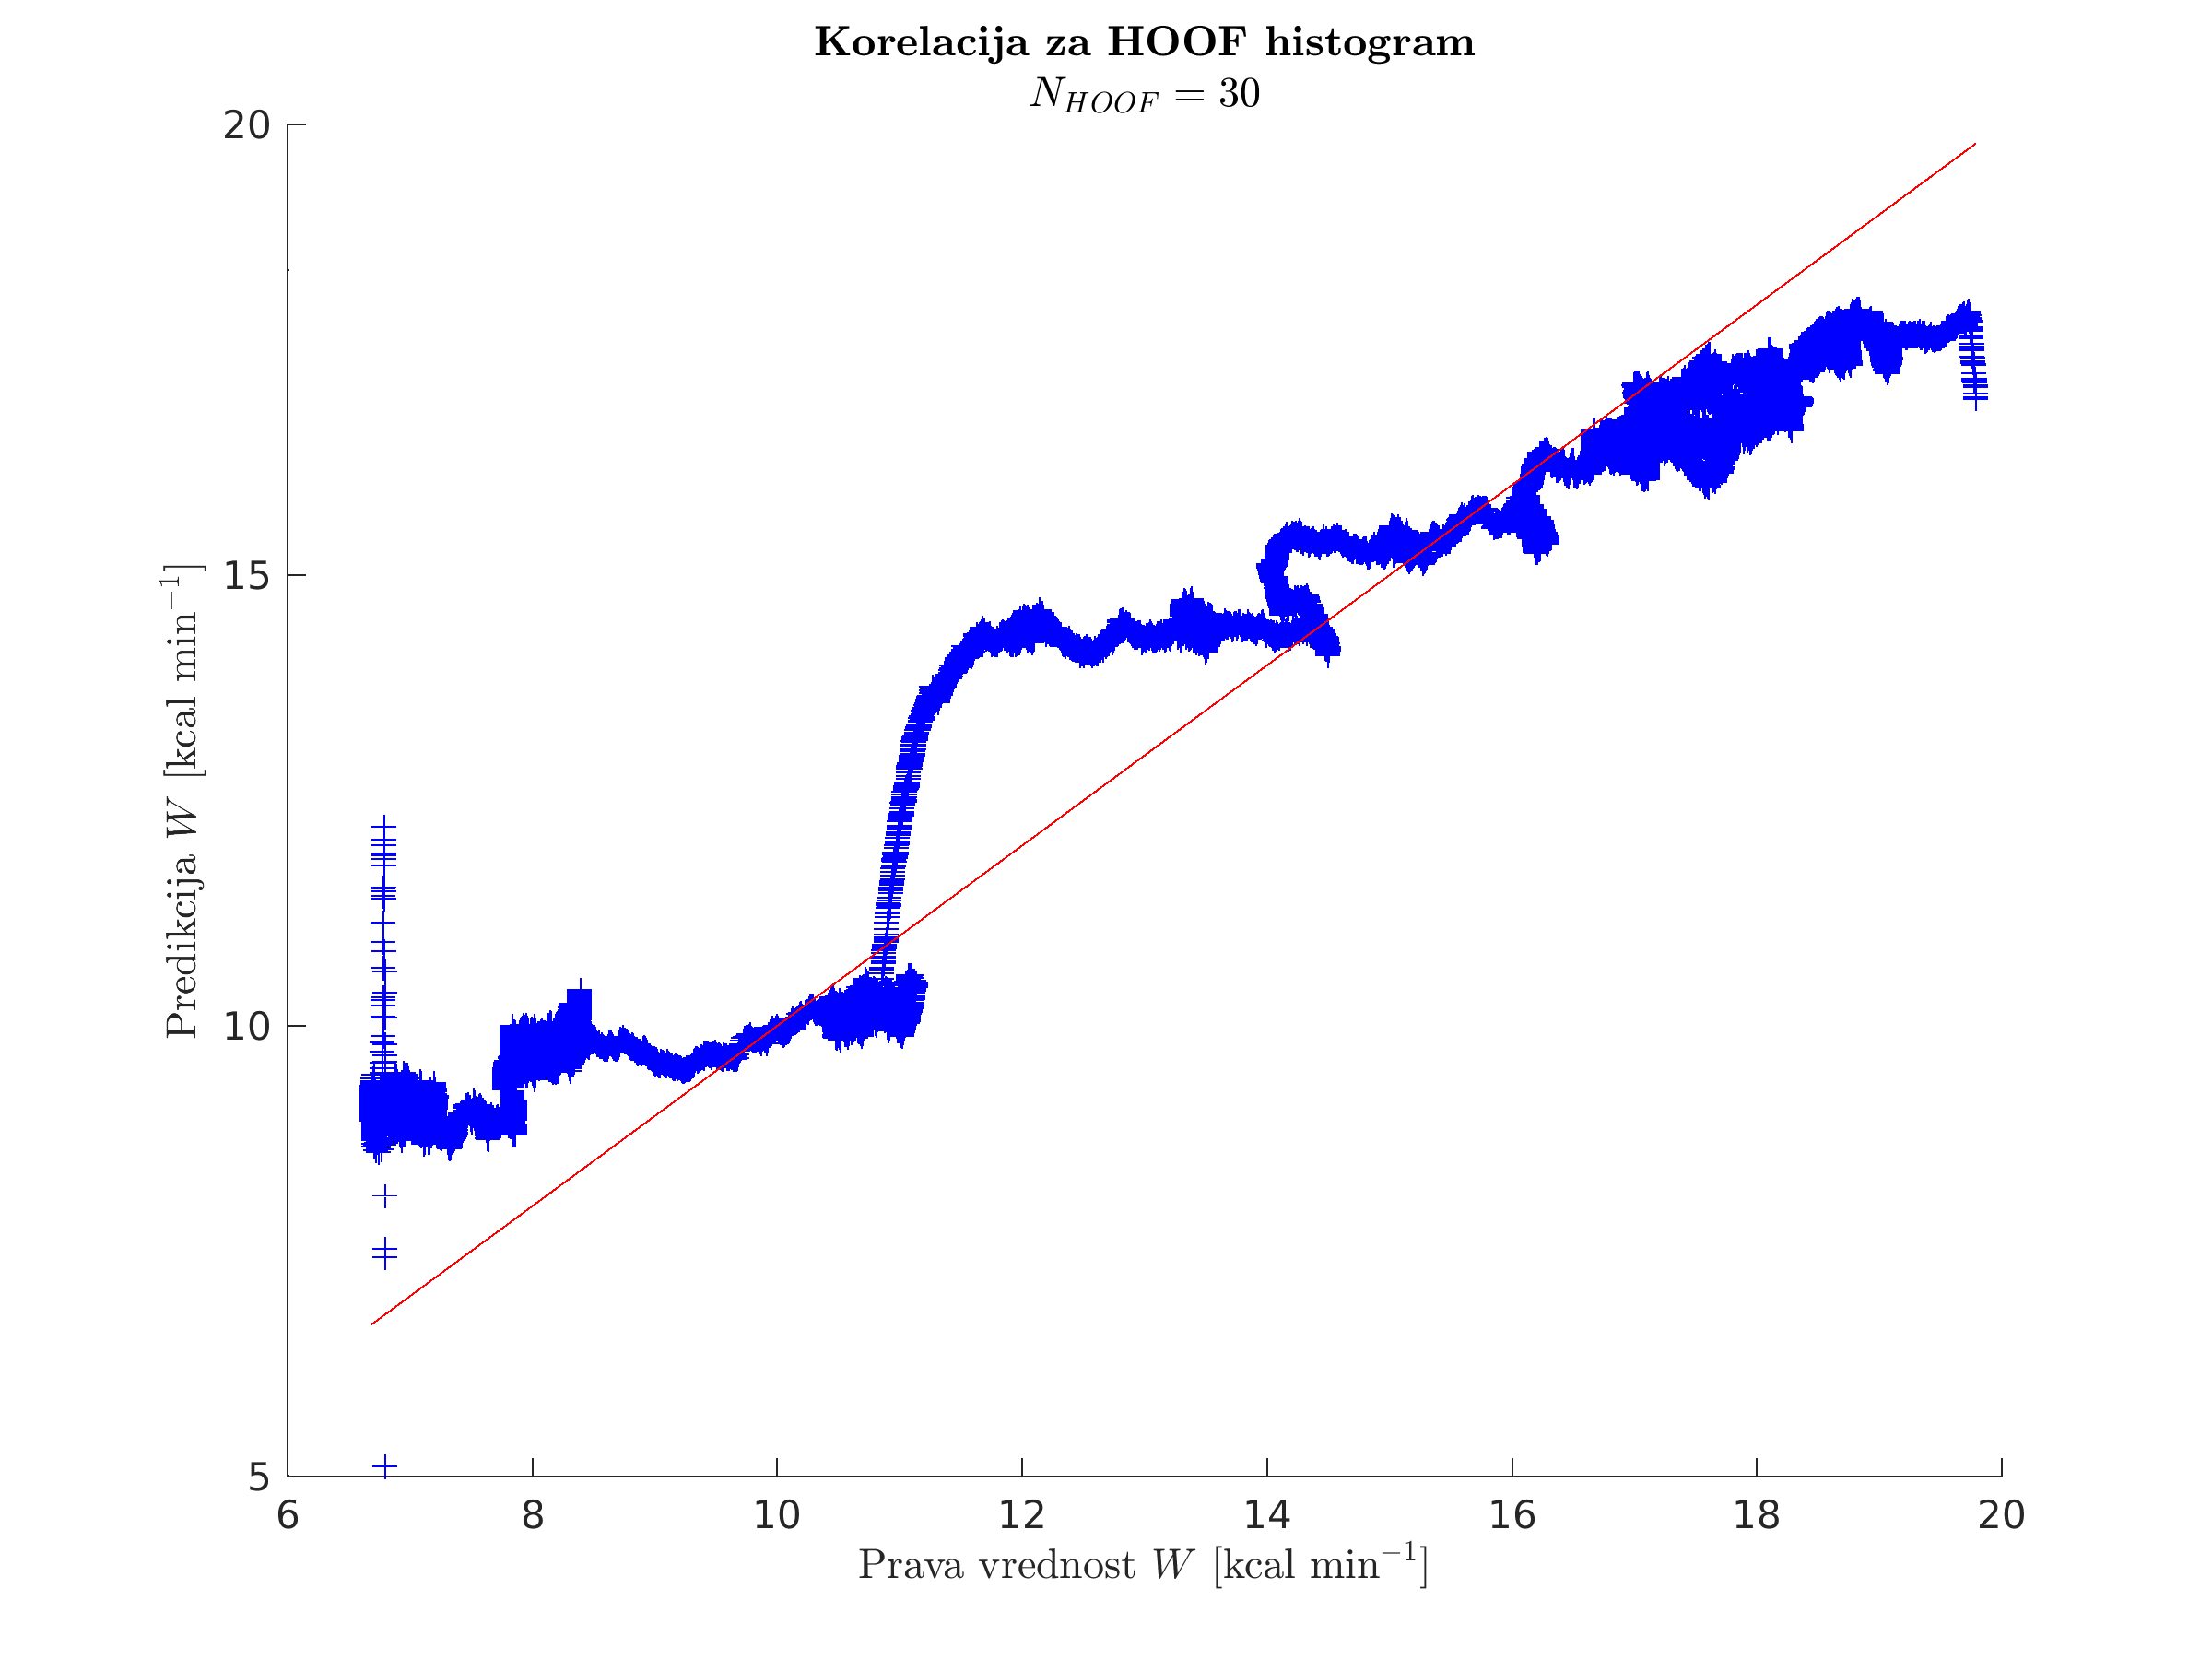
\includegraphics[width=\columnwidth]{./Slike/corr-hoof-30.png}
        \caption{Korelacija $N_{HOOF}=30$.}
        \label{fig:corr-hoof-30}
    \end{subfigure}
    ~
    \begin{subfigure}[t]{0.45\columnwidth}
      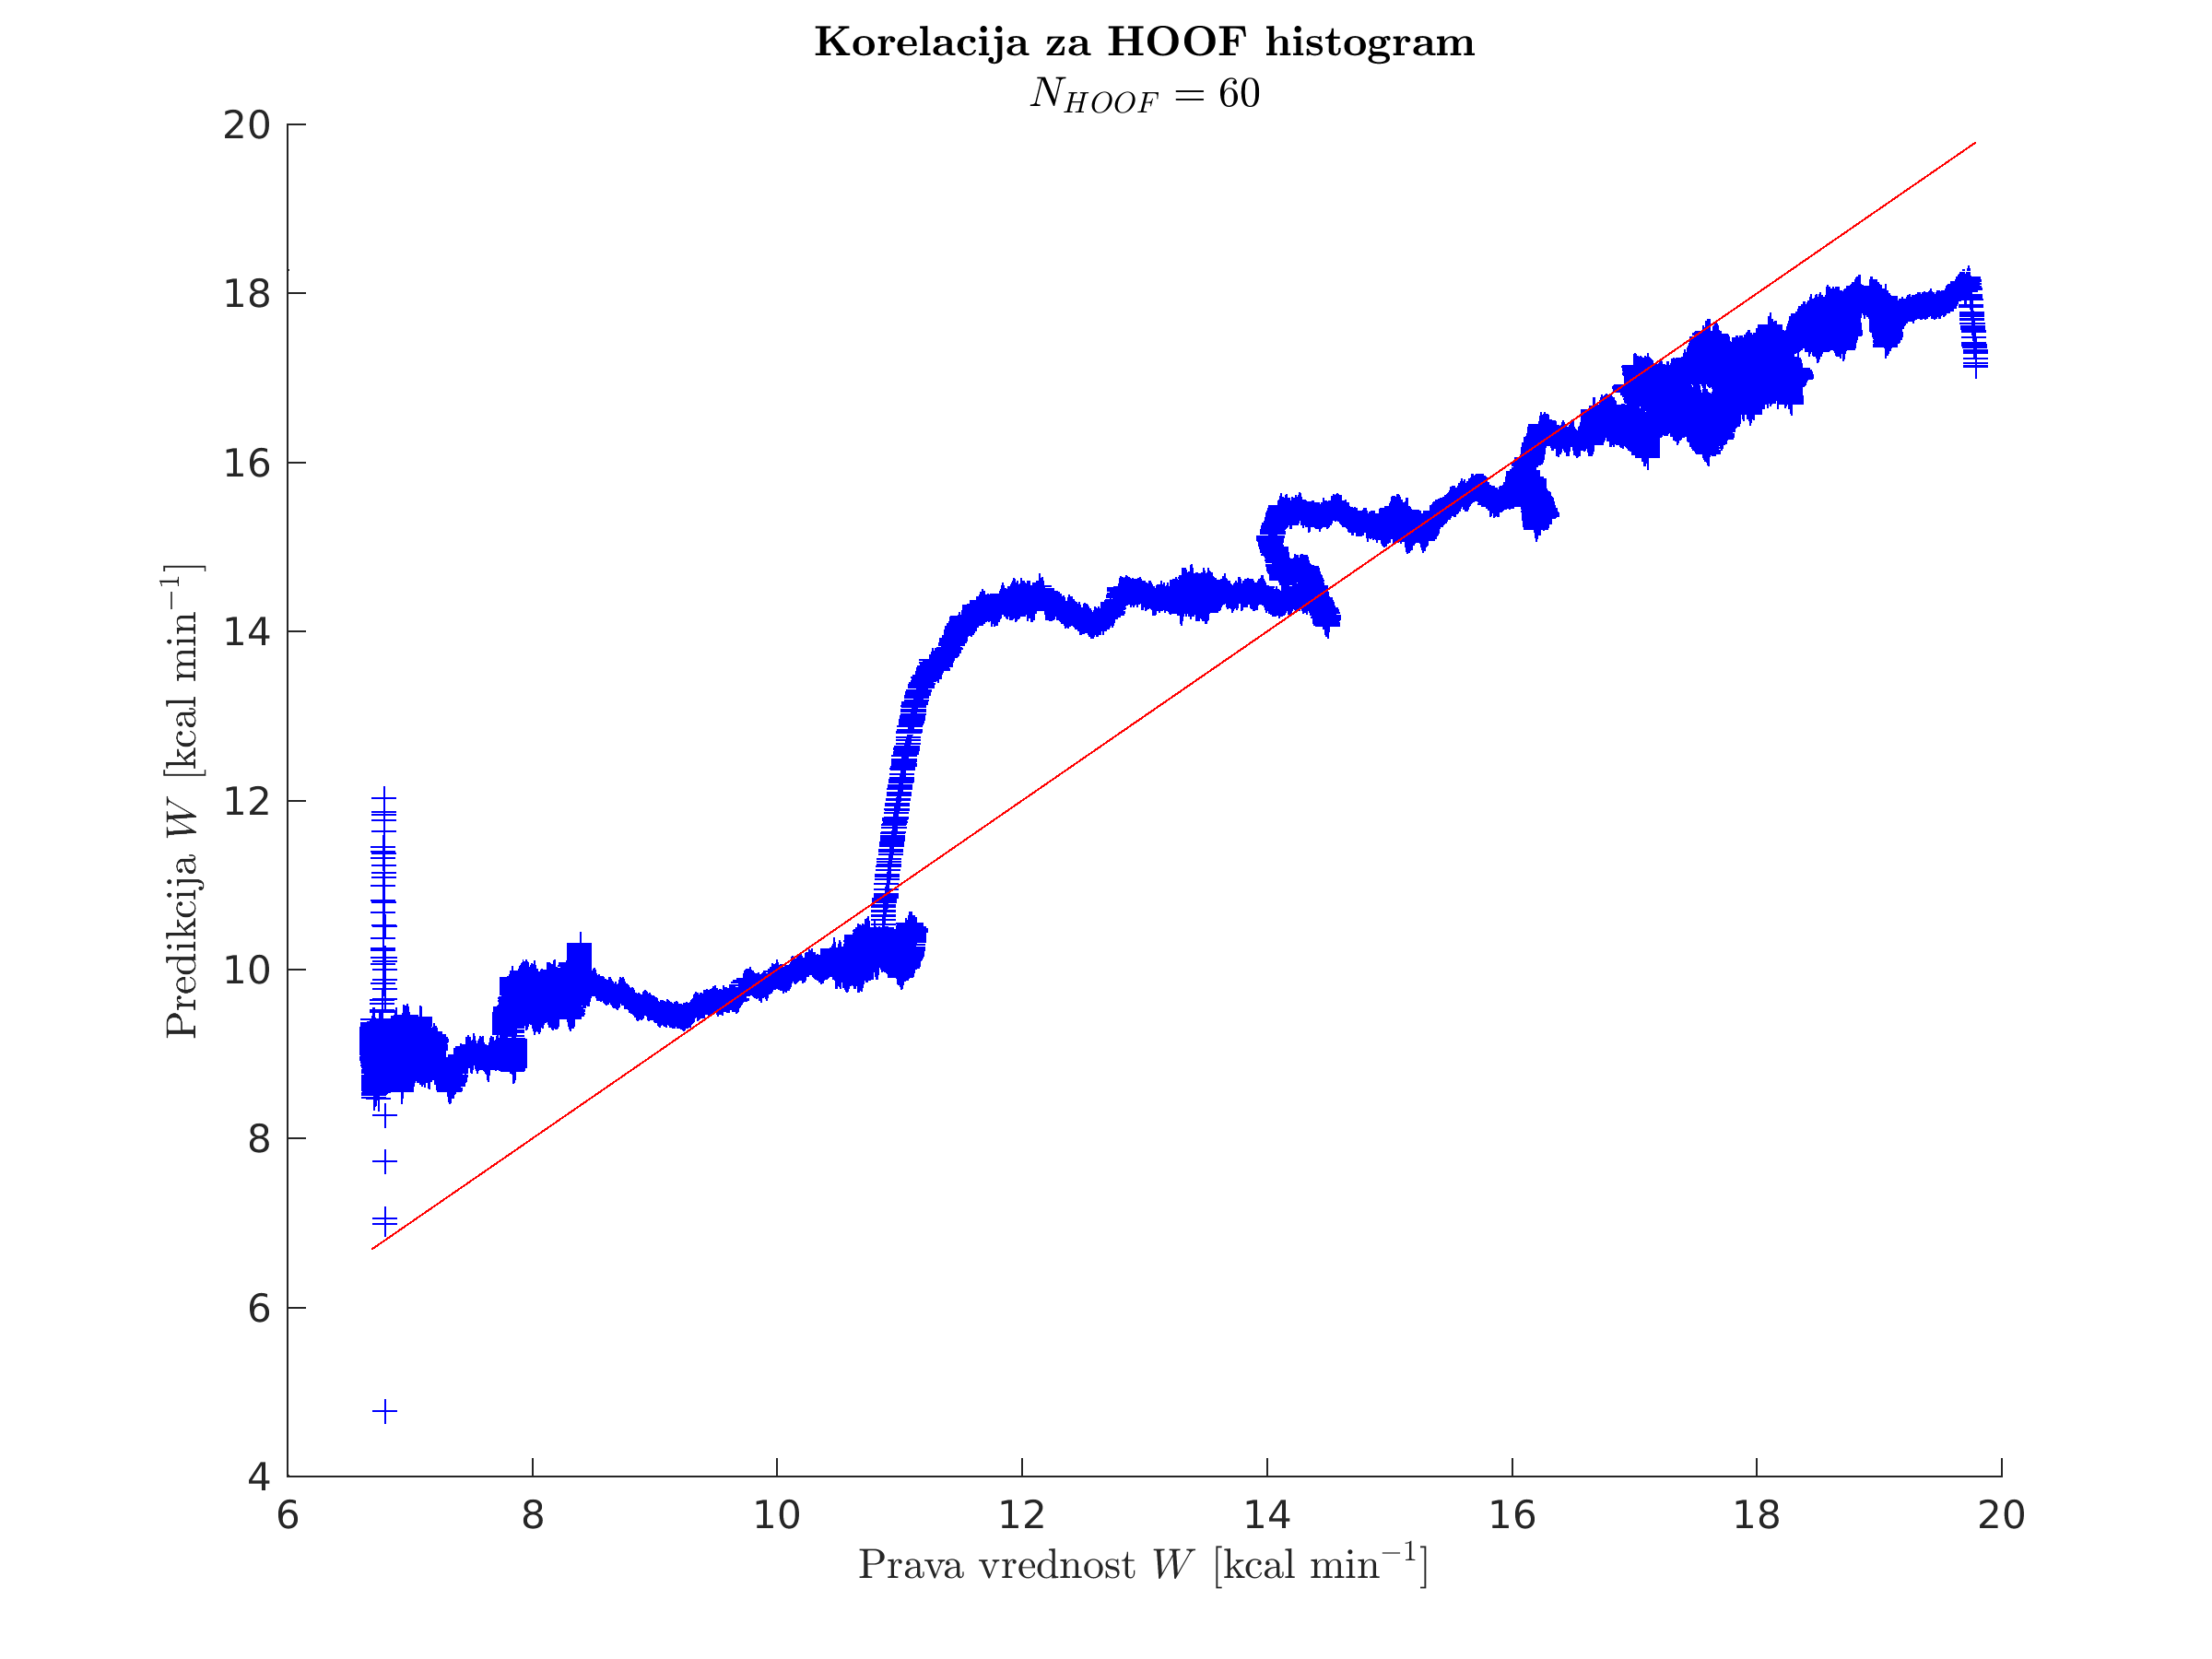
\includegraphics[width=\columnwidth]{./Slike/corr-hoof-60.png}
      \caption{Korelacija $N_{HOOF}=60$.}
      \label{fig:corr-hoof-60}
    \end{subfigure}
    ~
    \begin{subfigure}[b]{0.45\columnwidth}
      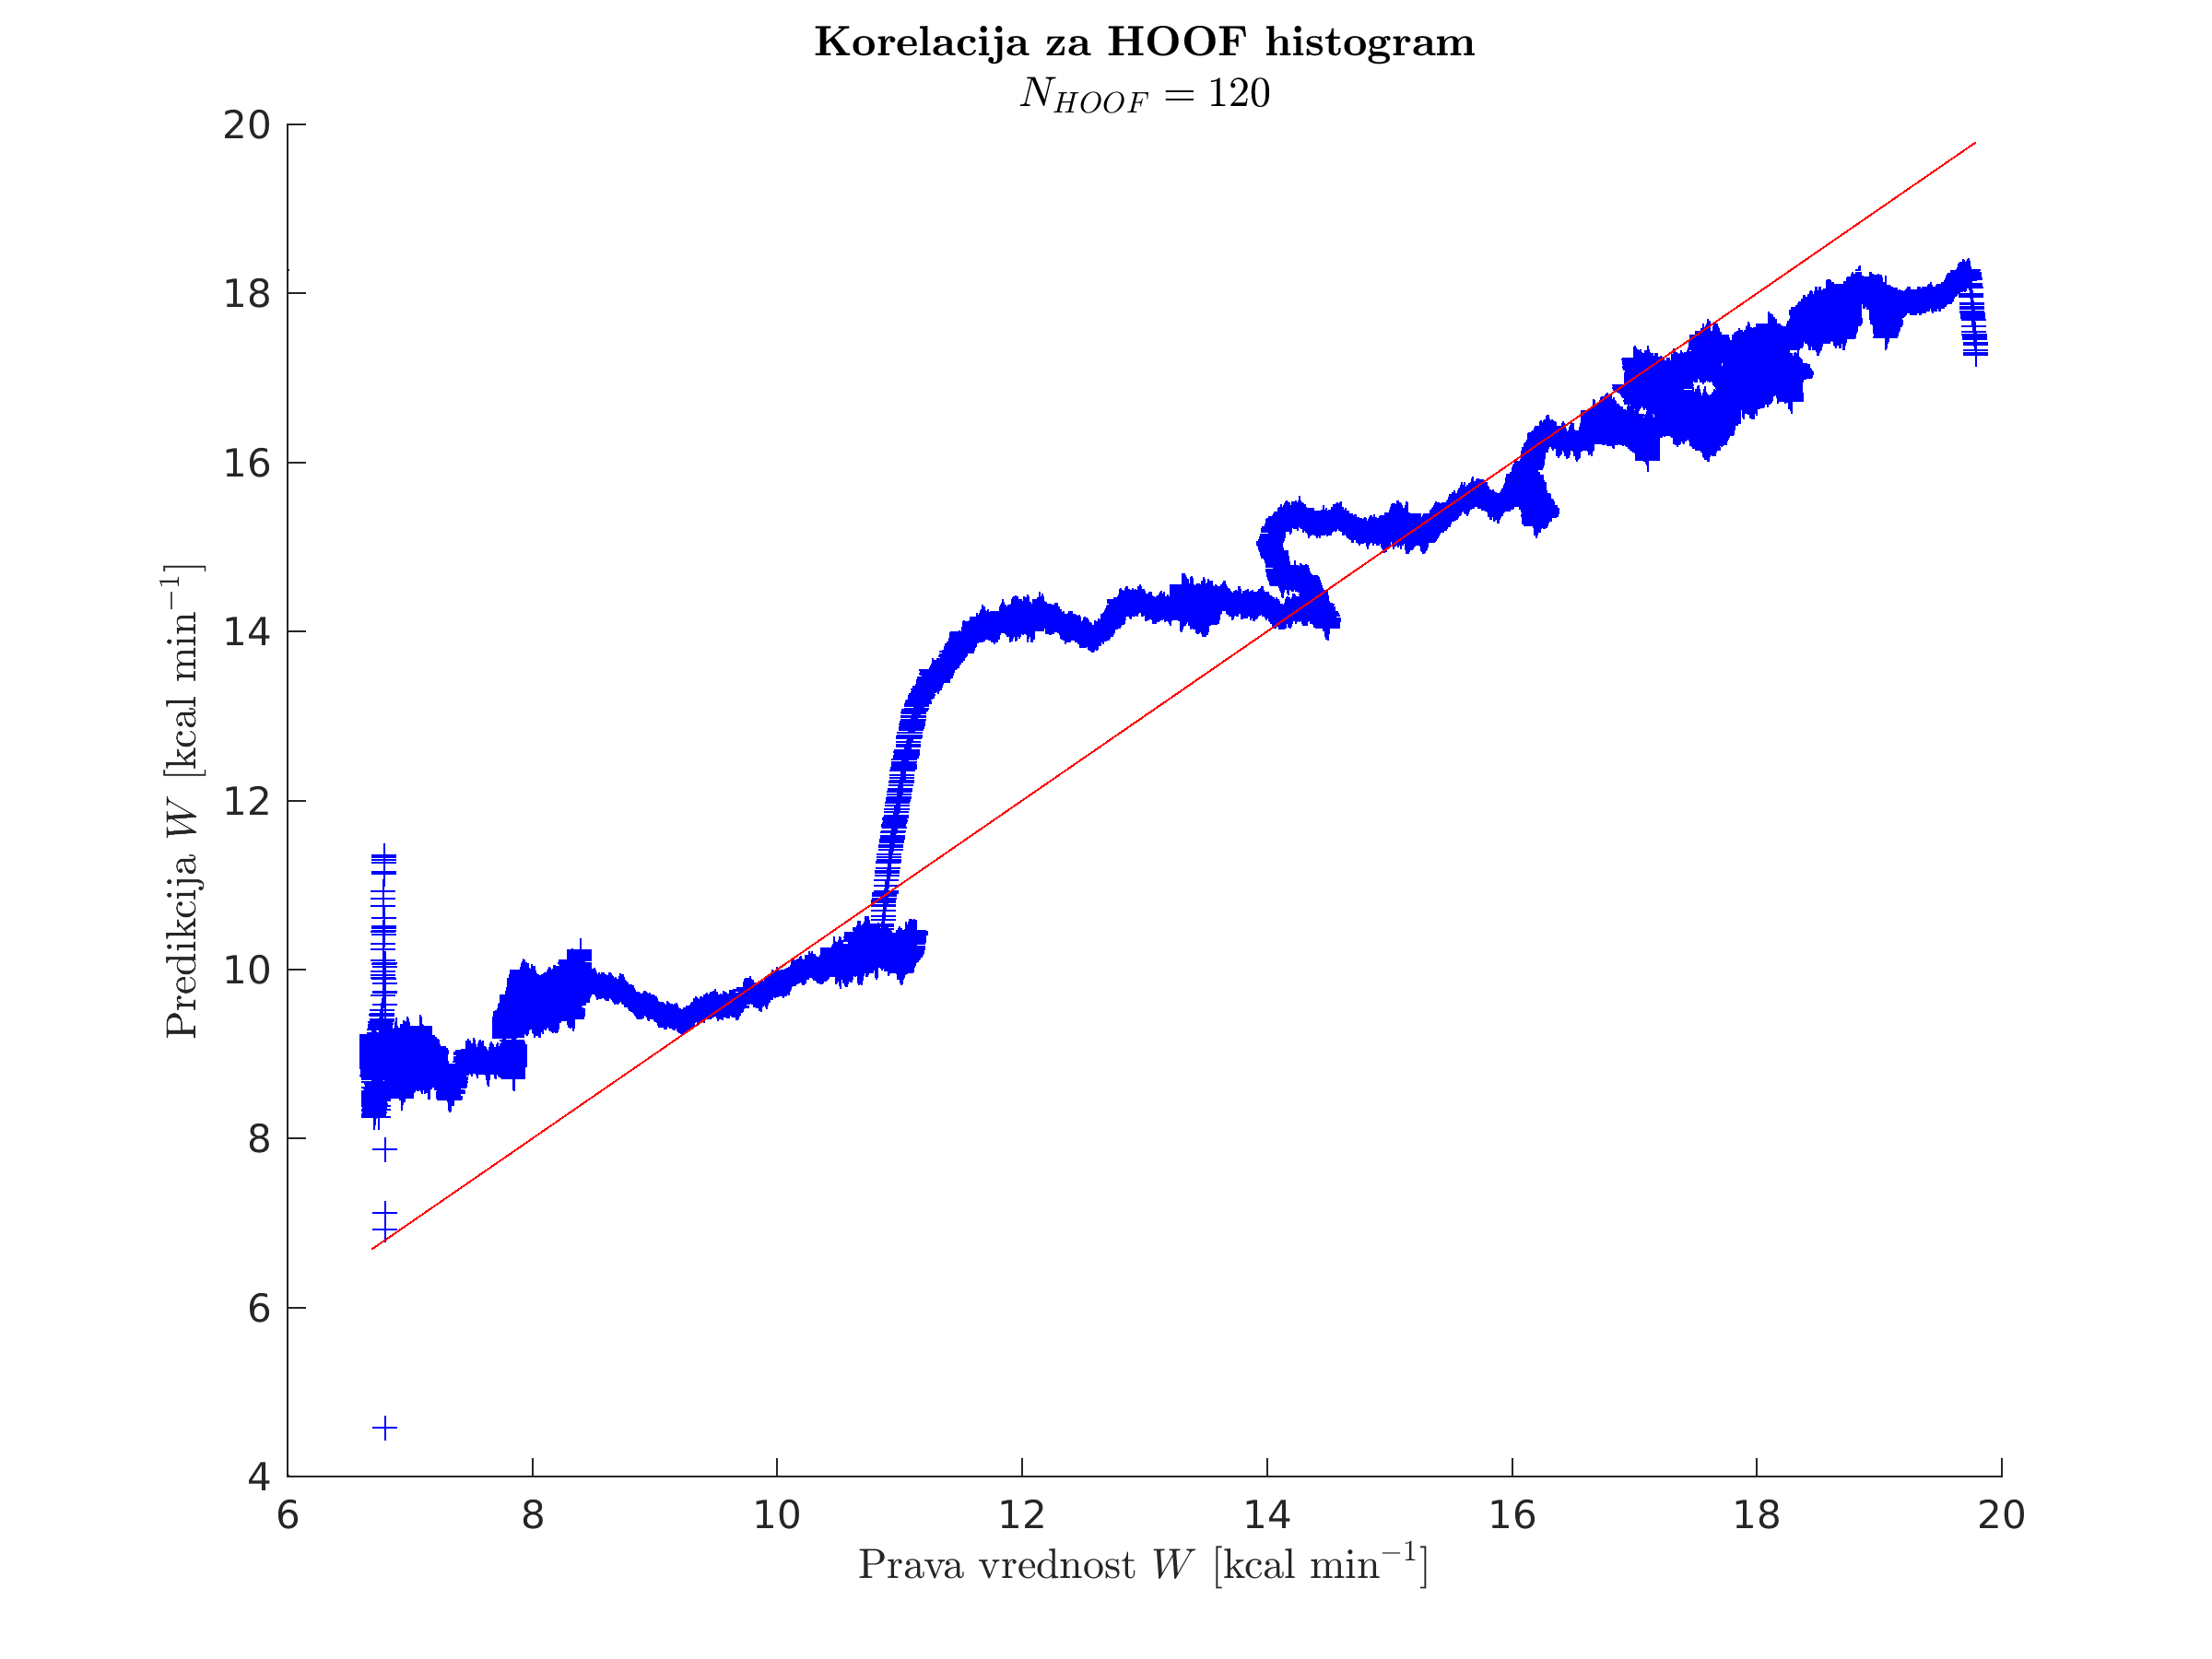
\includegraphics[width=\columnwidth]{./Slike/corr-hoof-120.png}
      \caption{Korelacija $N_{HOOF}=120$.}
      \label{fig:corr-hoof-120}
    \end{subfigure}
    ~
    \begin{subfigure}[b]{0.45\columnwidth}
      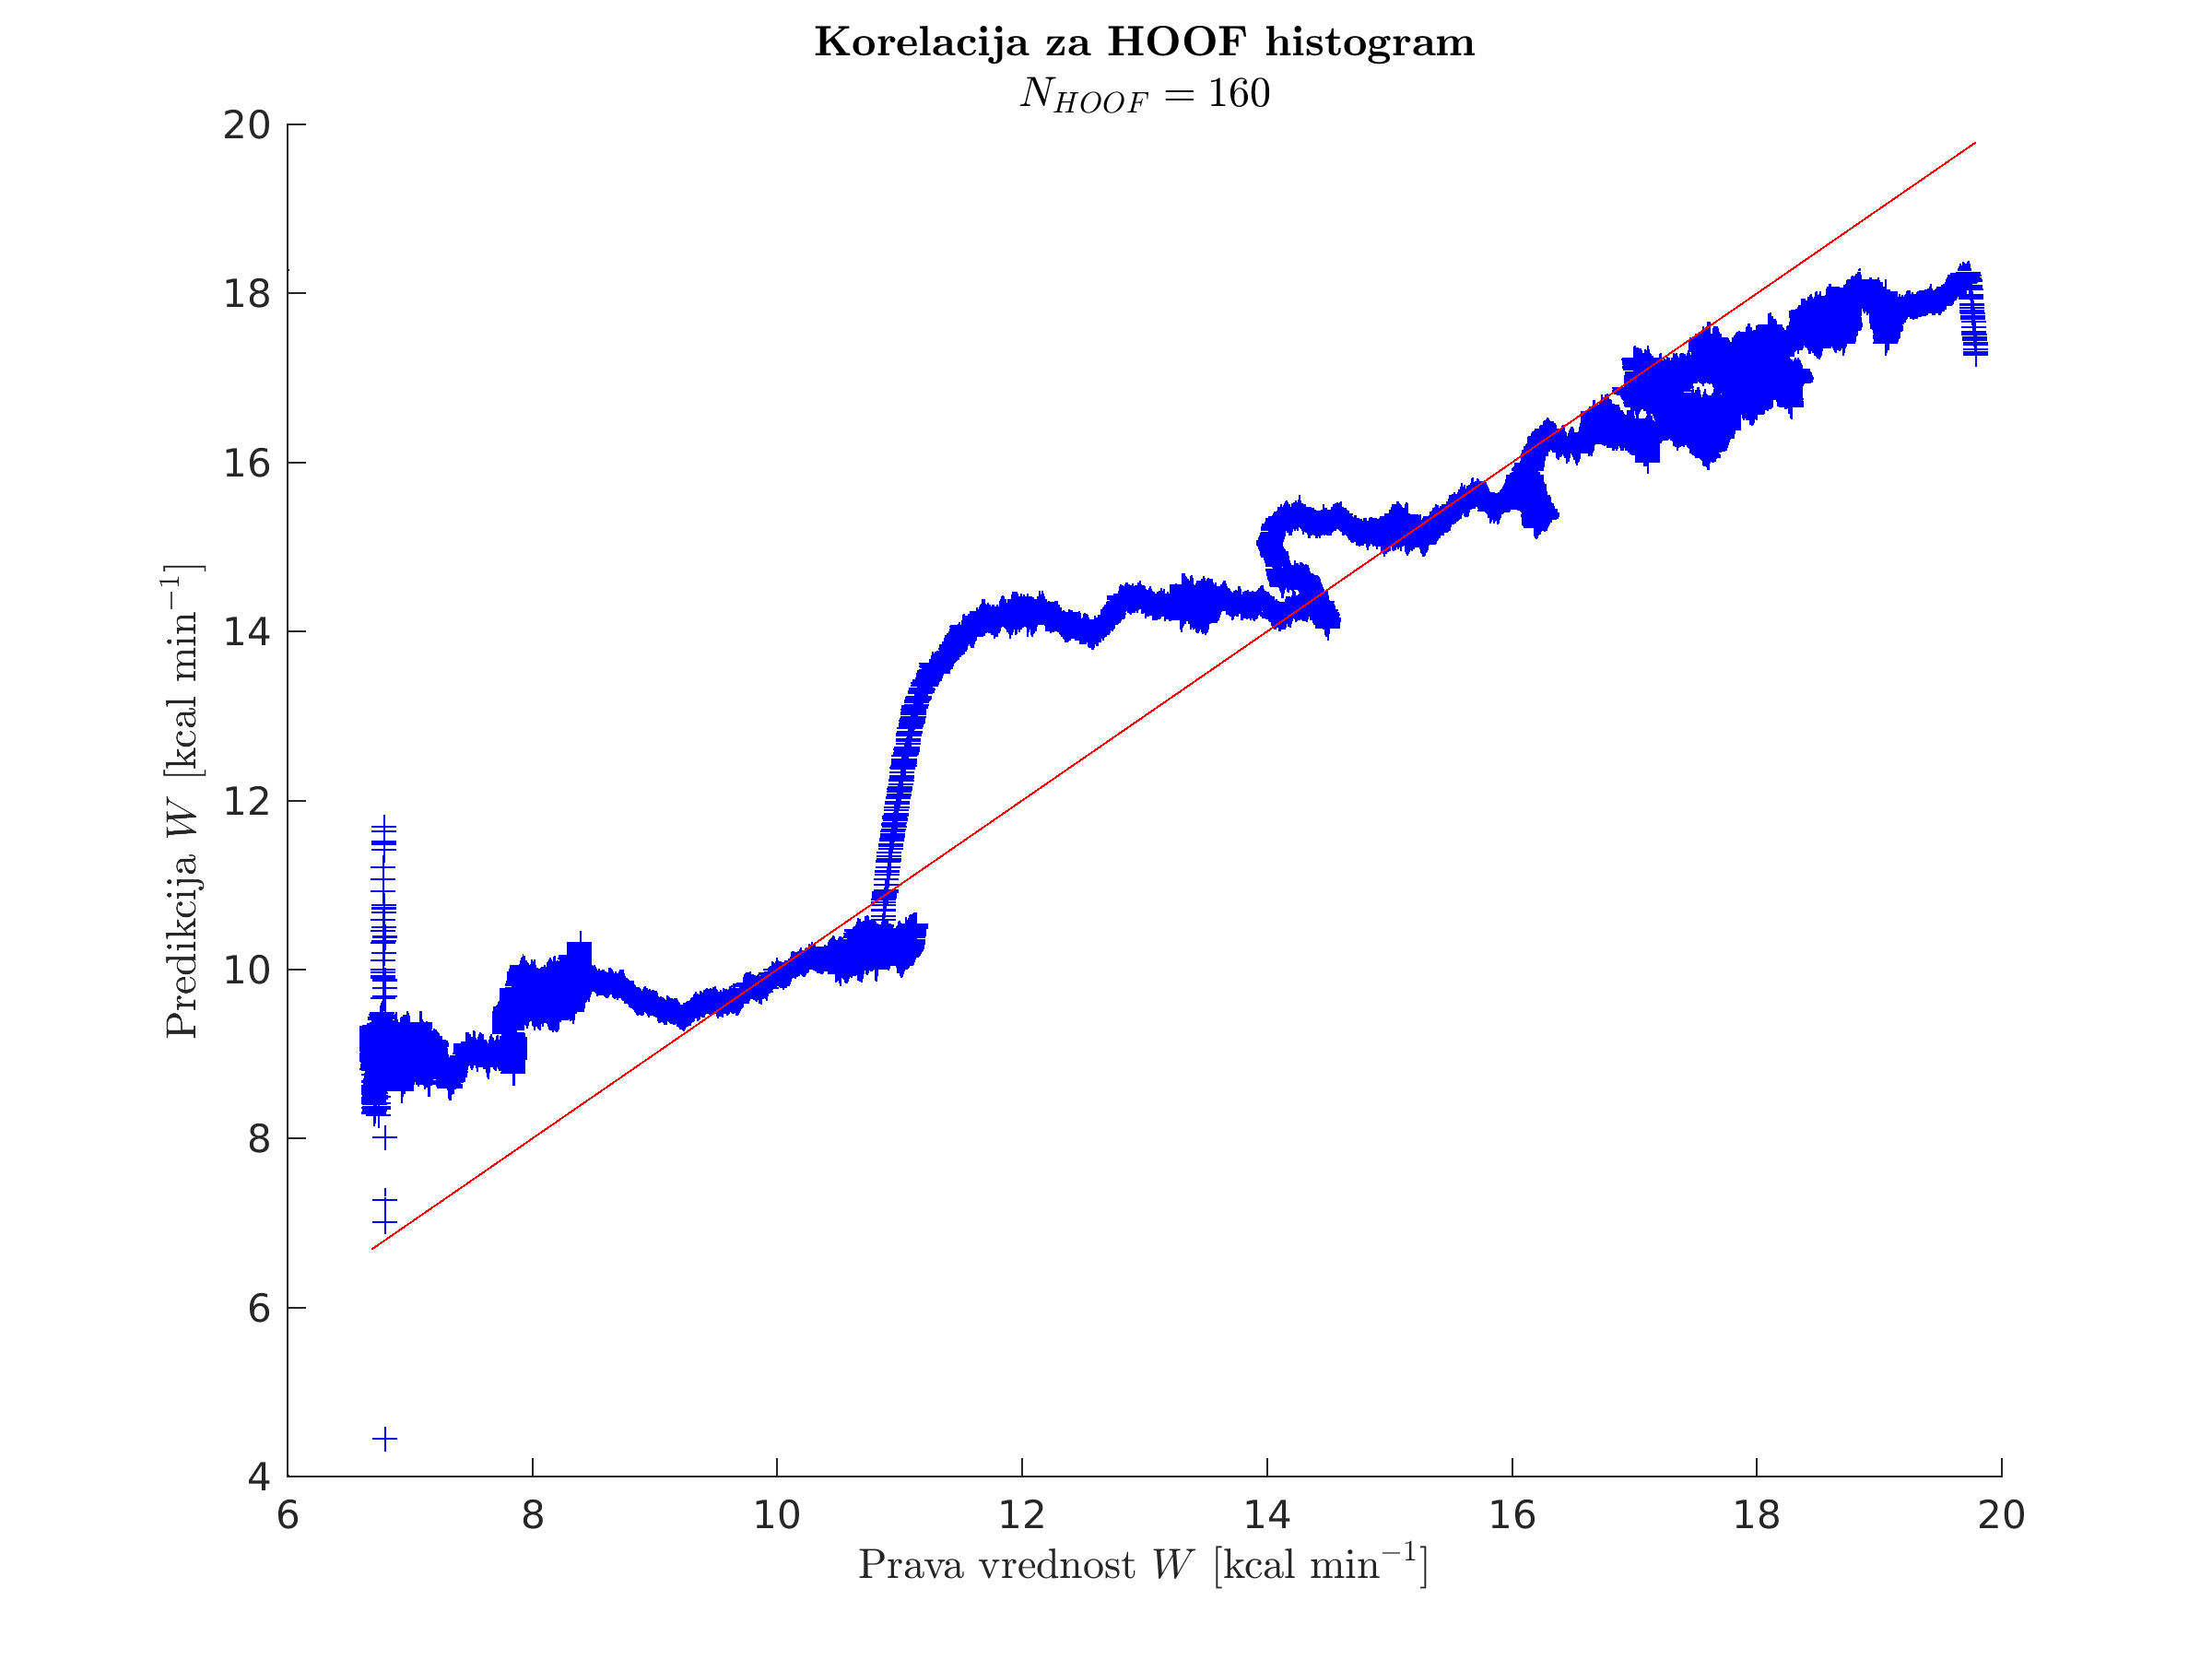
\includegraphics[width=\columnwidth]{./Slike/corr-hoof-160.png}
      \caption{Korelacija $N_{HOOF}=160$.}
      \label{fig:corr-hoof-160}
    \end{subfigure}
    \caption[Grafi korelacij modelov z različnim $N_{HOOF}$]{Grafi korelacij modelov z različnim številom stolpcev $N_{HOOF}$ HOOF deskriptorja. Rezultati so si zelo podobni.}
    \label{fig:corr-hoof}
\end{figure}









\subsection{Histogrami absolutnih tokovnih amplitud}\label{sec:hafa}
% Opis dodatnih deskriptorjev
% Kako uporabili nove deskriptorje
HOOF deskriptor modelira samo smer gibanja. Za modeliranje amplitude gibanja moramo uporabiti drug deskriptor. Idejo deskriptorja za modeliranje amplitude gibanja smo dobili v delu \cite{pers2010histograms}, kjer so avtorji za opis gibanja uporabili histograme optičnega toka (HOF). Gre za histograme v dveh dimenzijah, ki posebej kvantizirata amplitudo in smer optičnega toka v podregijah slike. 

Vektorju optičnega toka $\vec{w}$, ki je opredeljen v poglavju \ref{sec:hoof}, ima amplitudo določeno na intervalu \eqref{eq:interval-amp1}. 

\begin{equation}\label{eq:interval-amp1}
	[0, \infty)
\end{equation}


Interval \eqref{eq:interval-amp1} lahko kvantiziramo po enačbi \eqref{eq:interval-amp2}. Ta pomeni, da vektorju $\vec{w}$ določimo stolpec $b$, za katerega velja $1 \leq b \leq N_{HAFA}$, pri čemer je $N_{HAFA}$ celotno število stolpcev histograma na podlagi amplitude $\| \vec{w} \|$. S tako kvantizacijo omejimo zgornjo mejo intervala \eqref{eq:interval-amp1} na parameter histograma $N_{HAFA}$. Ko tak histogram normiramo, ga imenujemo histogram absolutnih tokovnih amplitud (HAFA). Določitev HAFA histograma je prikazan na sliki \ref{fig:hafa-histogram}.

\begin{equation}\label{eq:interval-amp2}
	\frac{b-1}{N_{HAFA}} \leq \| \vec{w} \| < \frac{b}{N_{HAFA}}
\end{equation}




\begin{figure}[htb]
\centering
\begin{tikzpicture}
% LAYERS
\pgfdeclarelayer{bg}
\pgfsetlayers{bg,main}

 % LENGTHS
\newcommand{\csl}{5}
\newcommand{\vl}{3}

\begin{pgfonlayer}{bg}
% Coordinate system
\begin{scope}
	\tikzset{vec/.append style = {
    	draw=teal!50!black!80,
        very thick
    }}
	\begin{polaraxis}[polar plot style]
		\addplot[vec, domain=0:1](20,x);
        \coordinate (v1) at (20, 0.7);
        \addplot[vec, domain=0:1.5](-45,x);
        \coordinate (v2) at (-45, 1);
        \addplot[vec, domain=0:0.5](160,x);
        \coordinate (v3) at (160,0.2);
	\end{polaraxis}
\end{scope}

\begin{scope}[xshift=10cm, yshift=0pt]
	\draw (0,1) rectangle (1,2) node (h1) [midway] {$ 0.5$};
    \draw (0,2) rectangle (1,3) node (h2) [midway] {$1$};
    \draw (0,3) rectangle (1,4) node (h3) [midway] {$1.5$};
    \node at (0,0) {HAFA stolpci};
\end{scope}
\end{pgfonlayer}

\tikzset{show/.style={
	->,
    >=stealth,
    very thick,
    line width=1mm,
    draw=red!50!black!50,
    shorten >=2mm
    }}
\draw [show] (v1) circle (1mm);
\draw [show] (v1) to[out=-90, in=180] (h2);
\draw [show] (v2) circle (1mm);
\draw [show] (v2) to[out=60, in=180] (h3);
\draw [show] (v3) circle (1mm);
\draw [show] (v3) to[out=-90, in=180] (h1);
\end{tikzpicture}

\caption[Prikaz določitve HAFA histograma glede na velikost vektorja]{Prikaz določitve HAFA histograma glede na velikost vektorja optičnega toka $\vec{u}$. Slika prikazuje določitev za $3$ stolpce.}
\label{fig:hafa-histogram}
\end{figure}





Parameter $N_{HAFA}$ smo določili na podlagi rezultatov evaluacije v tabeli \ref{tab:nhafa} in grafov korelacije med referenčnimi podatki in predikcijo \ref{fig:corr-hafa}. Za evaluacijo smo uporabili enak eksperimentalni protokol kot za HOOF značilke v poglavju \ref{sec:hoof}, s to razliko, da smo značilke normirali na intervalu $[0, 1]$ in odstranili stolpec z amplitudami $0.5$. S tem smo odstranili šum, ki se je pojavil, ko ni bilo nobenega gibanja. Amplitudo šuma smo določili, kot maksimalno vrednost amplitude, ki še ni predstavljala gibanja. Optimalni parametri evaluacijske metode so predstavljeni v tabeli \ref{tab:nhafa-param}.


\begin{table}[htb]
	\centering
    \begin{tabular}{S[table-format=2.0] S[table-format=2.3] S[table-format=1.3]  S[table-format=1.3] S[table-format=1.3]}
    \toprule
    \thead{$\mathbf{N_{HAFA}}$} & \thead{$\mathbf{C}$} & \thead{$\mathbf{\gamma}$} & \thead{$\mathbf{\epsilon}$} & \thead{MSE} \\ 
    \midrule
    30 & 8 & 5.657 & 0.616 & 4.329 \\
    60 & 8 & 5.657 & 0.616 & 4.327 \\
    120 & 8 & 5.657 & 0.616 & 4.327 \\
    160 & 8 & 5.657 & 0.616 & 4.327 \\
    \bottomrule
    \end{tabular}
    \caption[Optimalni parameteri RBF jedra modelov za določitev $N_{HAFA}$]{Optimalni parametri RBF jedra za modele z različnim številom stolpcev $N_{HAFA}$ v HAFA deskriptorju.}
    \label{tab:nhafa-param}
\end{table}

V tabeli \ref{tab:nhafa} lahko vidimo, da so rezultati praktično enaki. Za našo metodo smo izbrali $N_{HAFA}=60$, kar v grobem predstavlja $60$ različnih hitrosti z maksimalno amplitudo \SI{60}{px.f^{-1}}.

\begin{table}[htb]
	\centering
    \begin{tabular}{S[table-format=2.0] S[table-format=1.3] S[table-format=1.3] S[table-format=1.3] S[table-format=2.2]}
    \toprule
    \thead{$N_{HAFA}$} & \thead{$r$} & \thead{RAE} & \thead{RMSE} & \thead{nSV [\%]}\\
    \midrule%nSV
    30 & 0.984 & 0.213 & 0.231 & 62.08 \\%17879/28799
    \boldentry{2.0}{60} & \boldentry{1.3}{0.984} & \boldentry{1.3}{0.211} & \boldentry{1.3}{0.228} & \boldentry{2.2}{62.60} \\%18028
    120 & 0.984 & 0.211 & 0.228 & 62.63 \\%18037
    160 & 0.984 & 0.211 & 0.228 & 62.63 \\%18037
    \bottomrule
    \end{tabular}
    \caption[Rezultati evaluacije modelov z različnim $N_{HAFA}$]{Rezultati evaluacije modelov z različnim številom stolpcev $N_{HAFA}$ HAFA deskriptorja. Optimalni rezultati so odebeljeni.}
    \label{tab:nhafa}
\end{table}

\begin{figure}[htb]
	\centering
    \begin{subfigure}[t]{0.45\columnwidth}
    	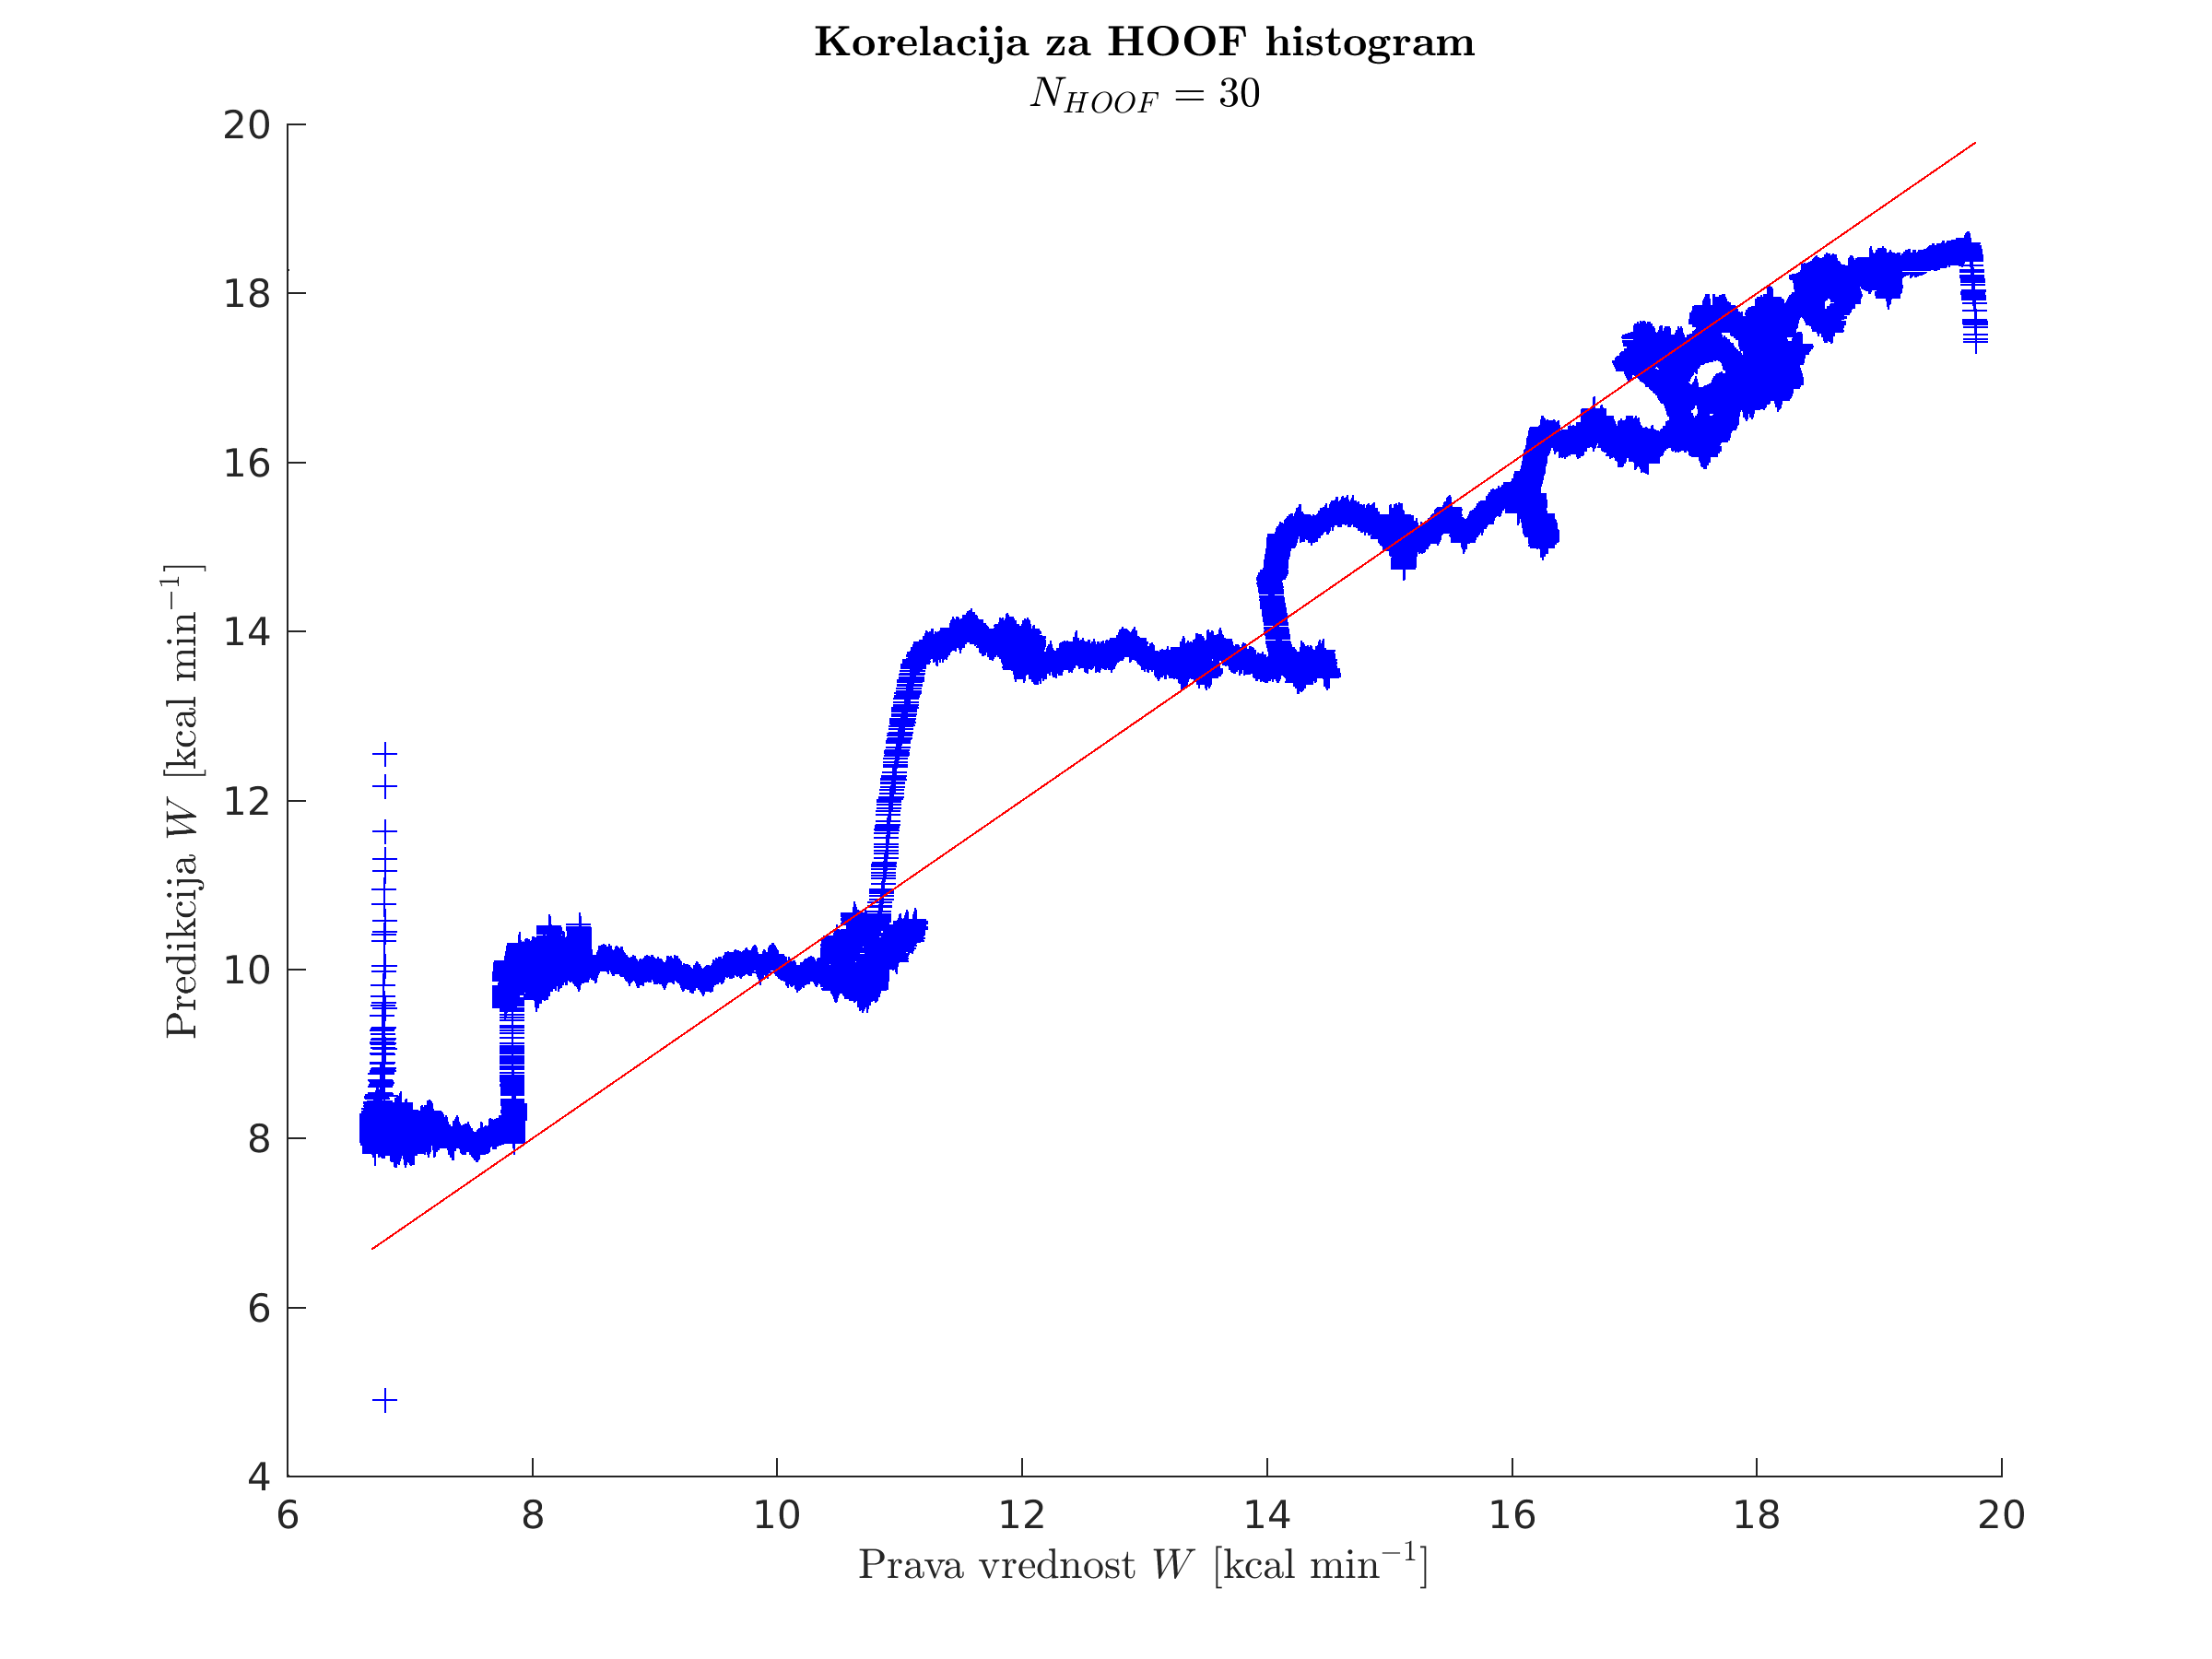
\includegraphics[width=\columnwidth]{./Slike/corr-hafa-30.png}
        \caption{Korelacija $N_{HAFA}=30$.}
        \label{fig:corr-hafa-30}
    \end{subfigure}
    ~
    \begin{subfigure}[t]{0.45\columnwidth}
      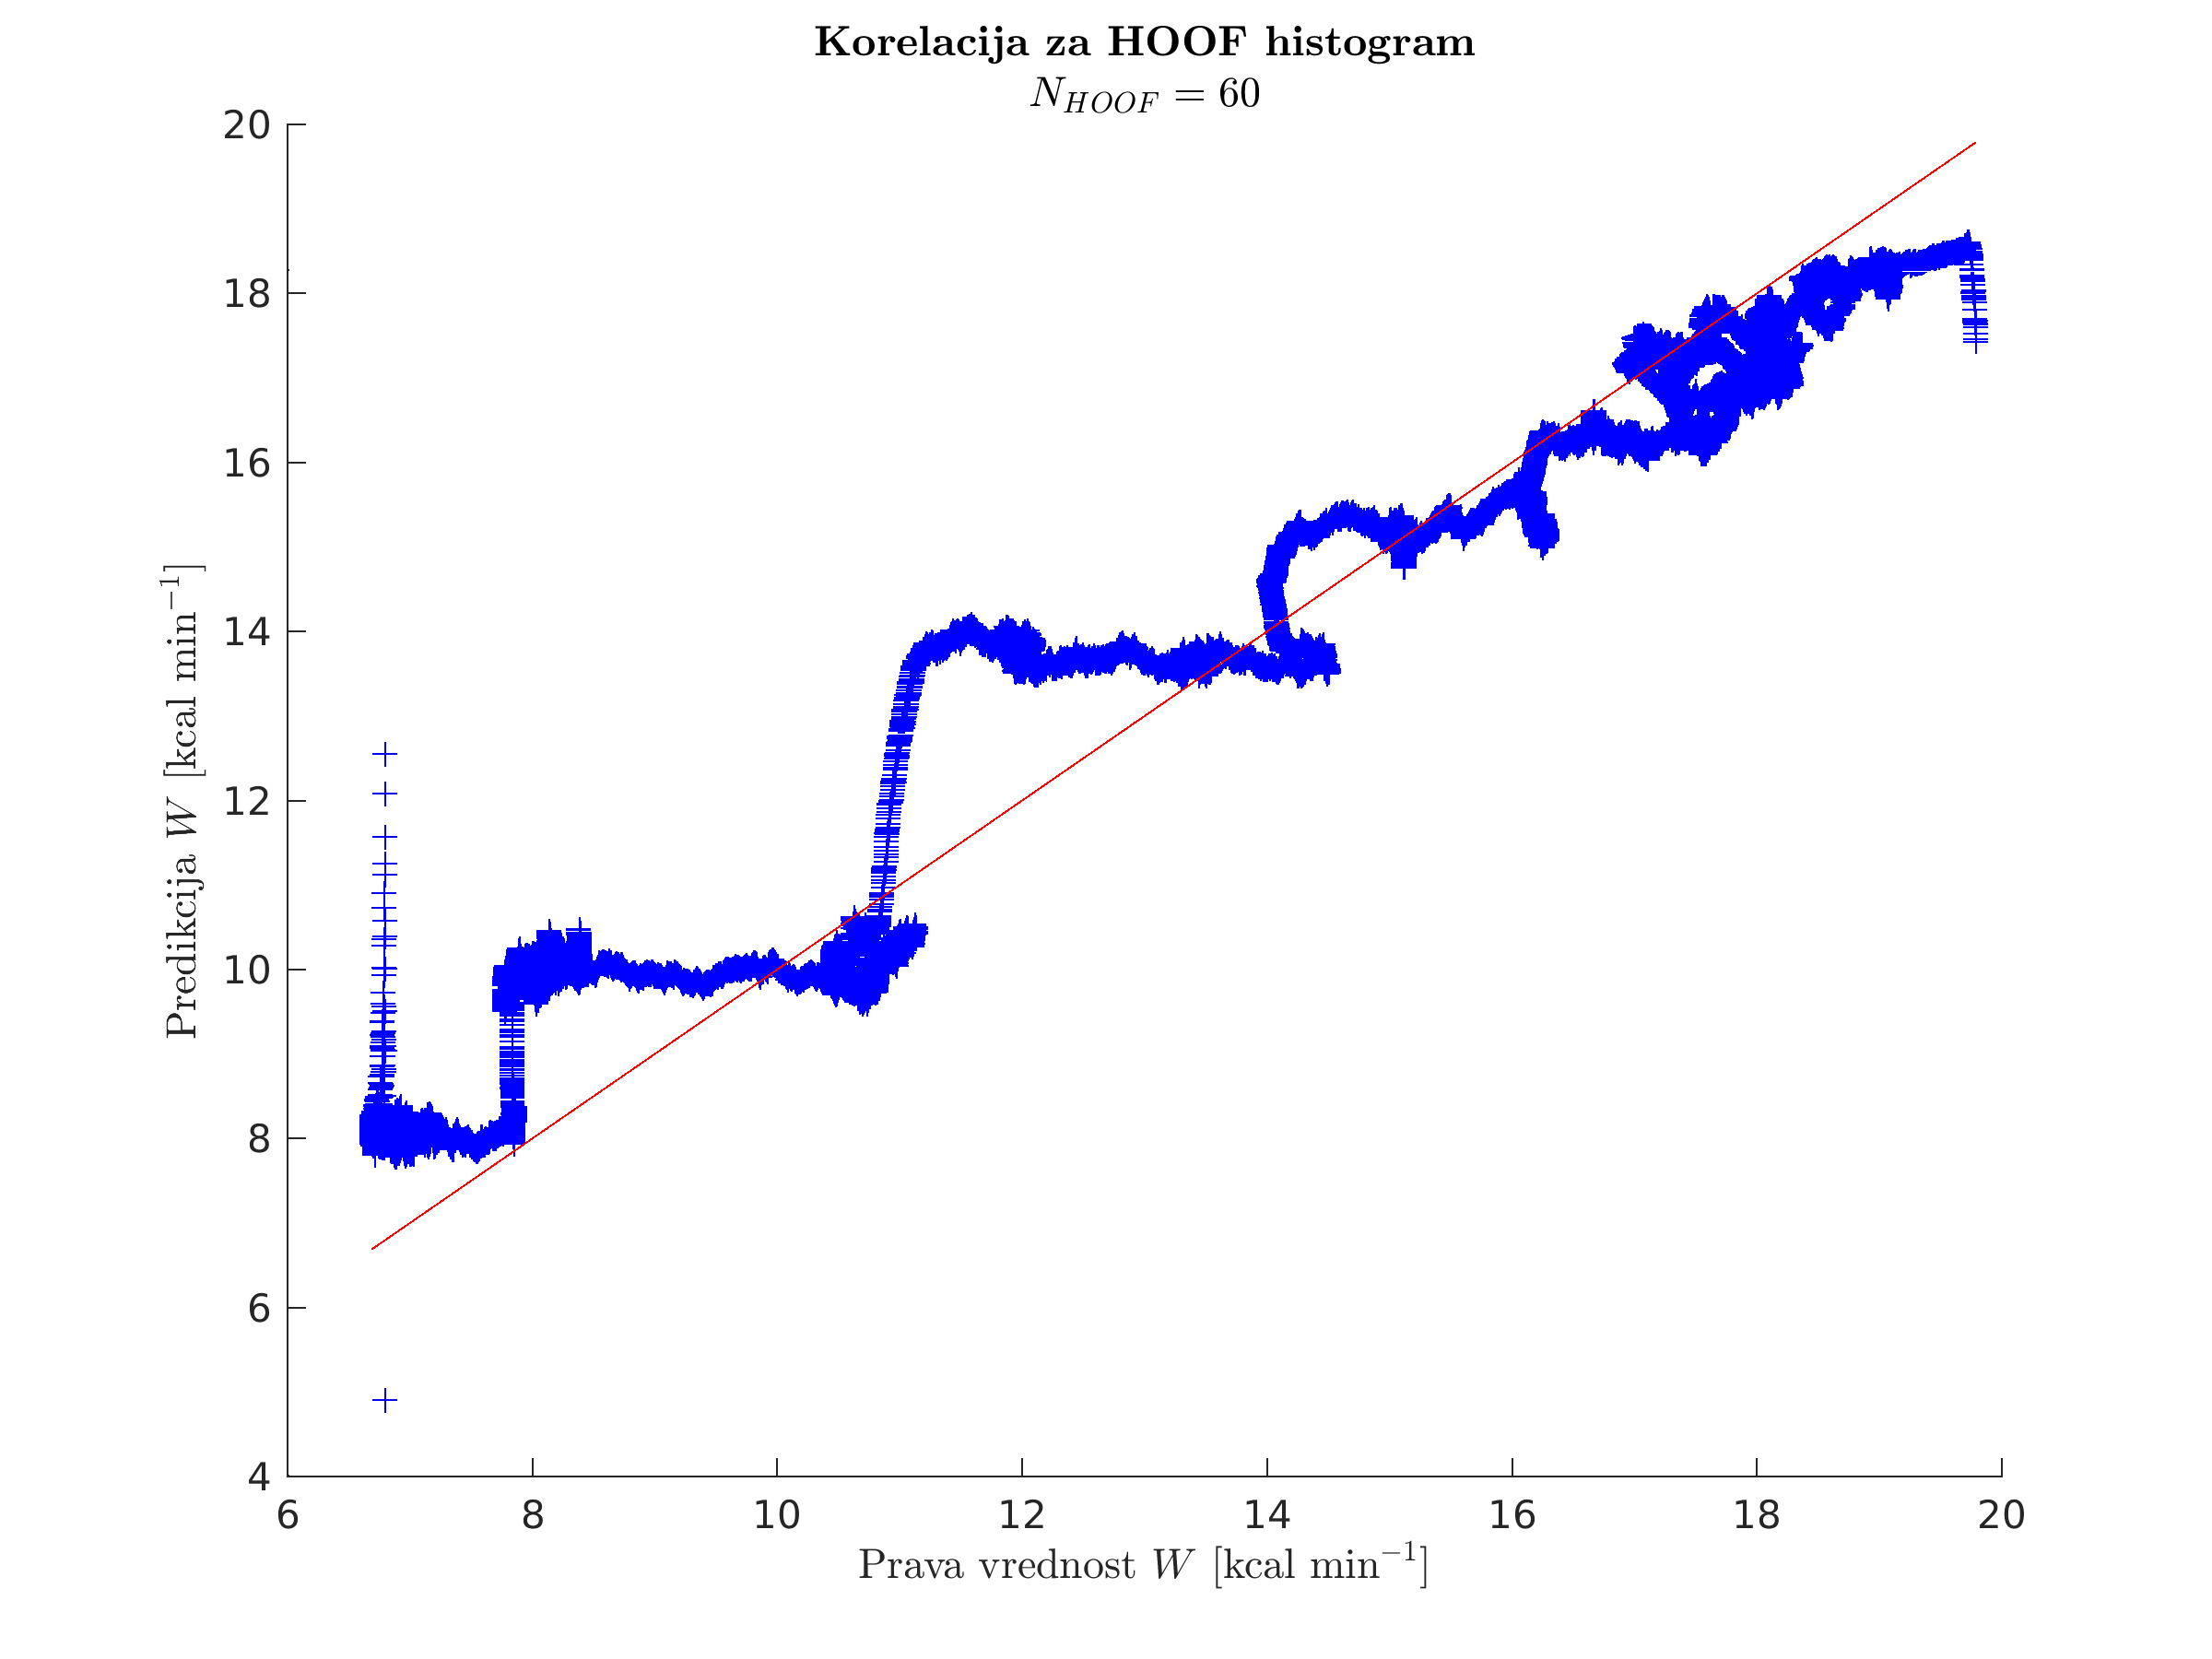
\includegraphics[width=\columnwidth]{./Slike/corr-hafa-60.png}
      \caption{Korelacija $N_{HAFA}=60$.}
      \label{fig:corr-hafa-60}
    \end{subfigure}
    ~
    \begin{subfigure}[b]{0.45\columnwidth}
      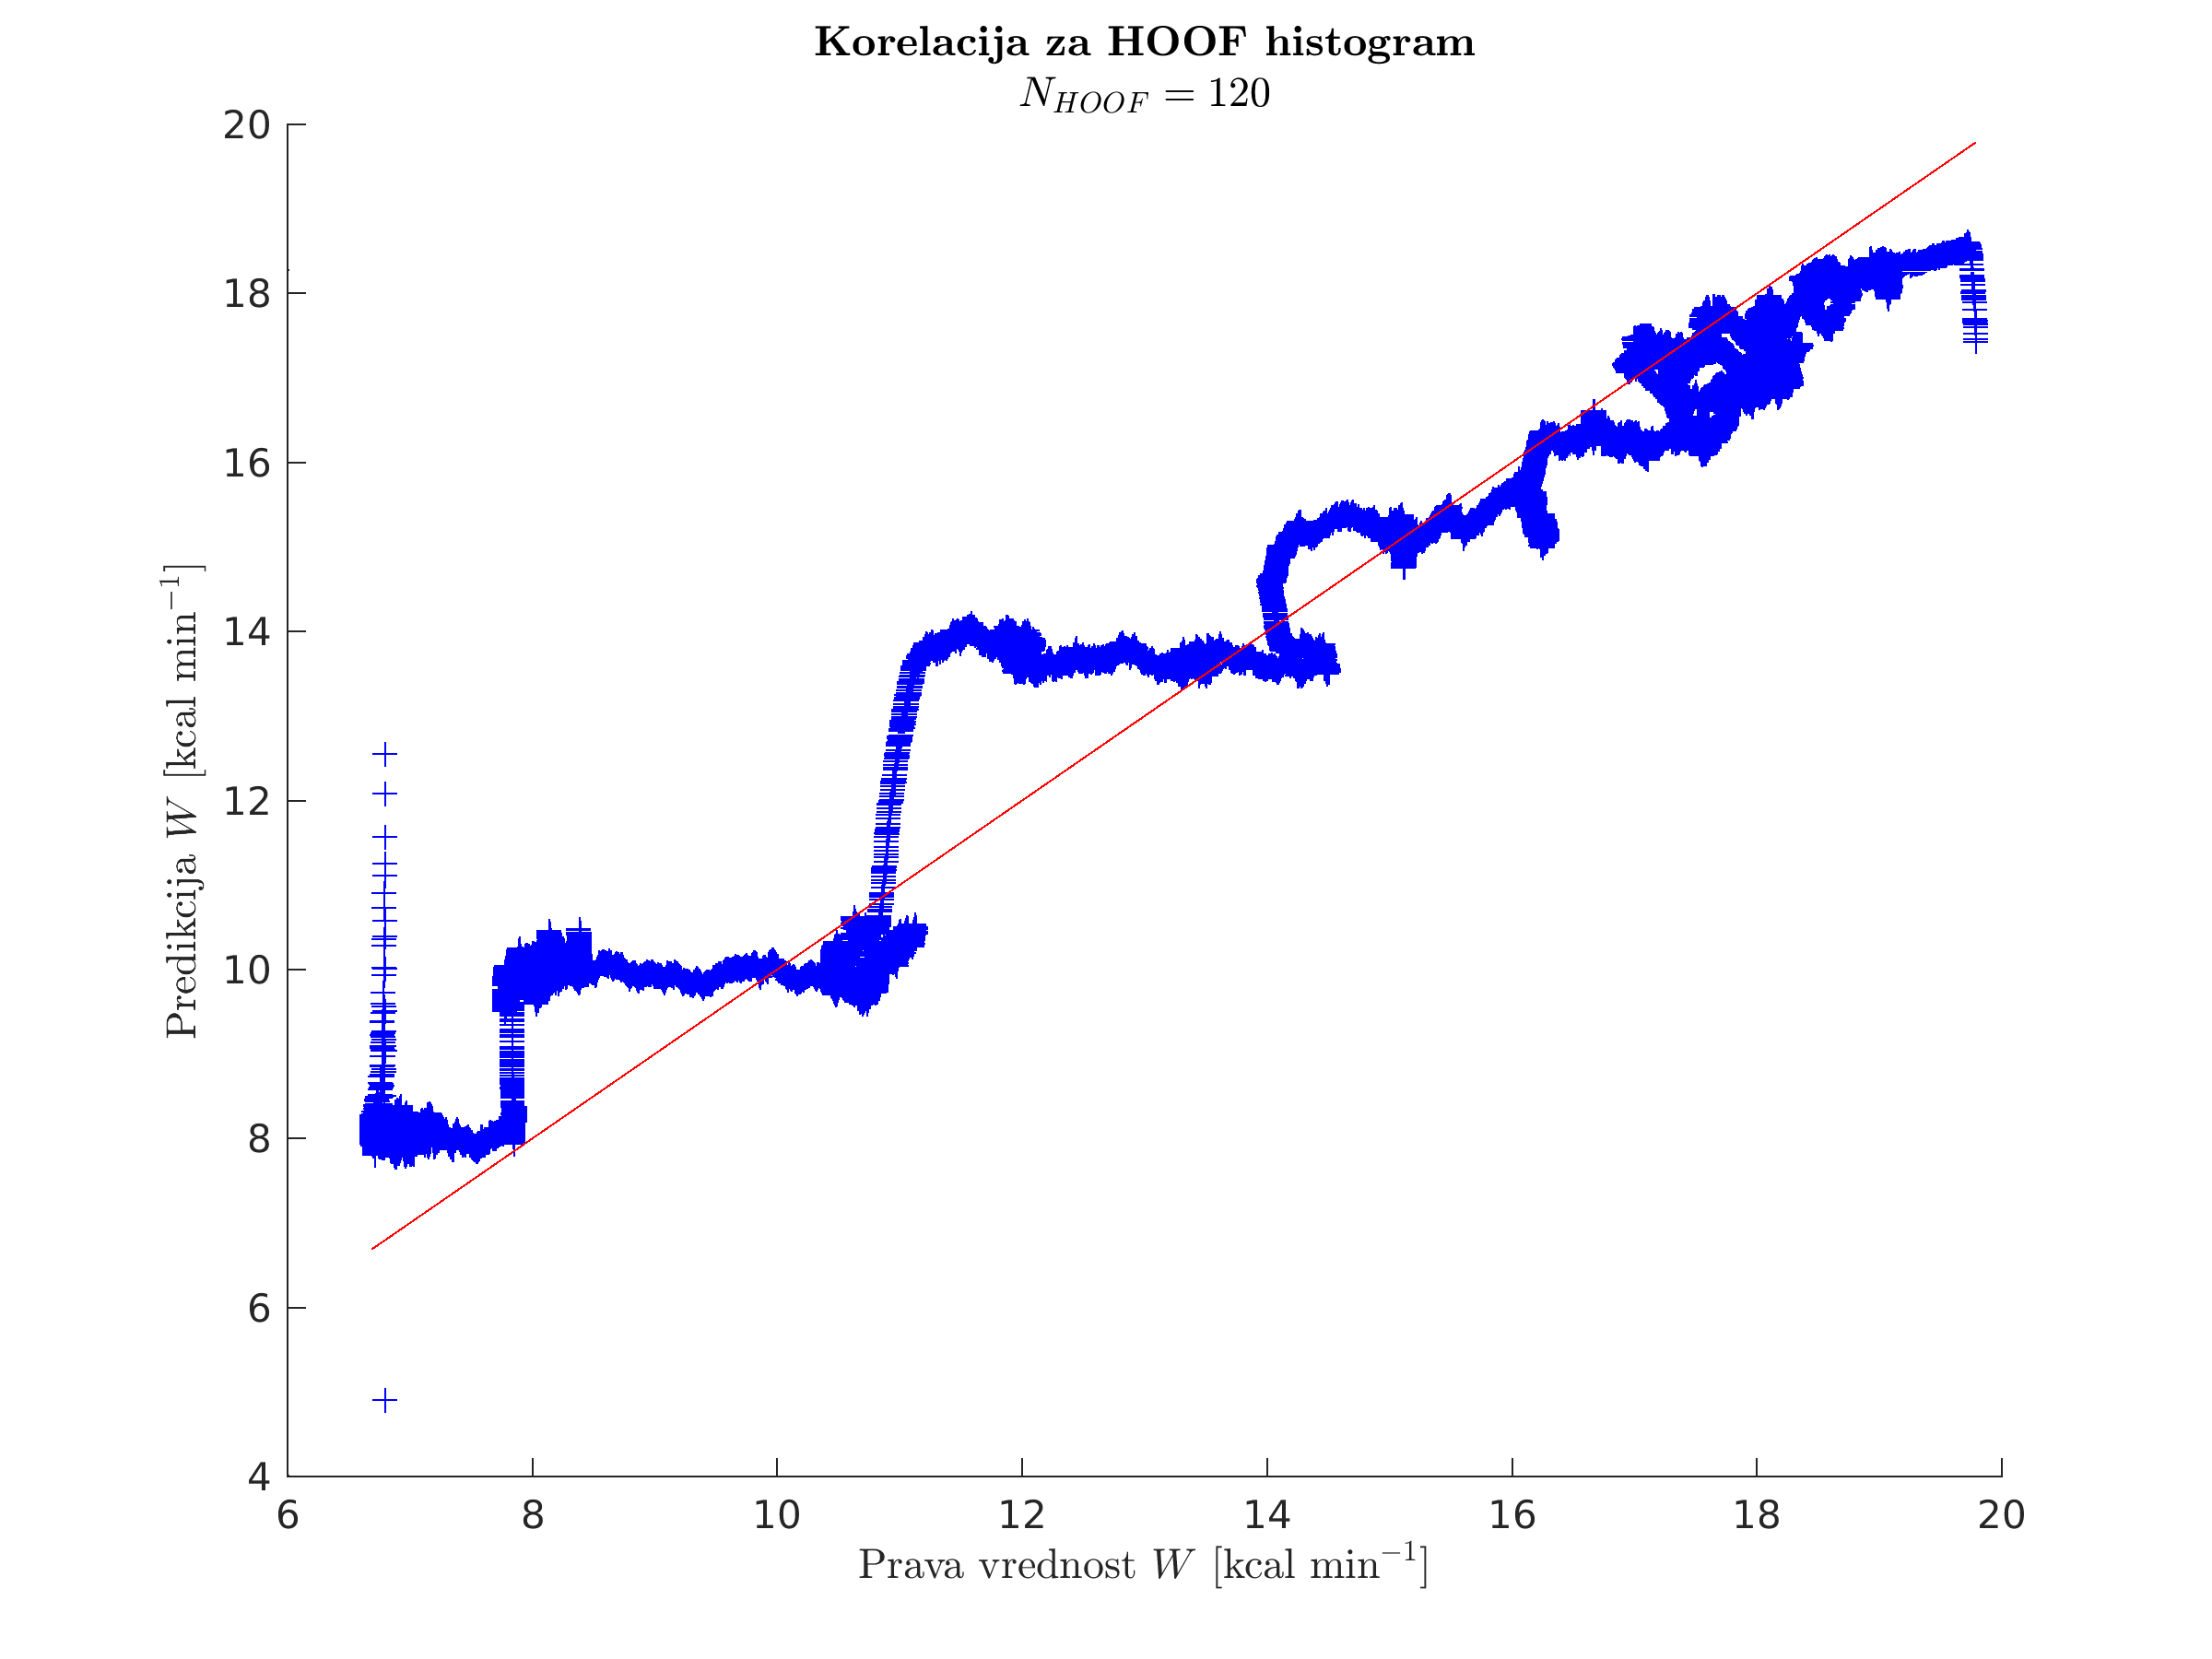
\includegraphics[width=\columnwidth]{./Slike/corr-hafa-120.png}
      \caption{Korelacija $N_{HAFA}=120$.}
      \label{fig:corr-hafa-120}
    \end{subfigure}
    ~
    \begin{subfigure}[b]{0.45\columnwidth}
      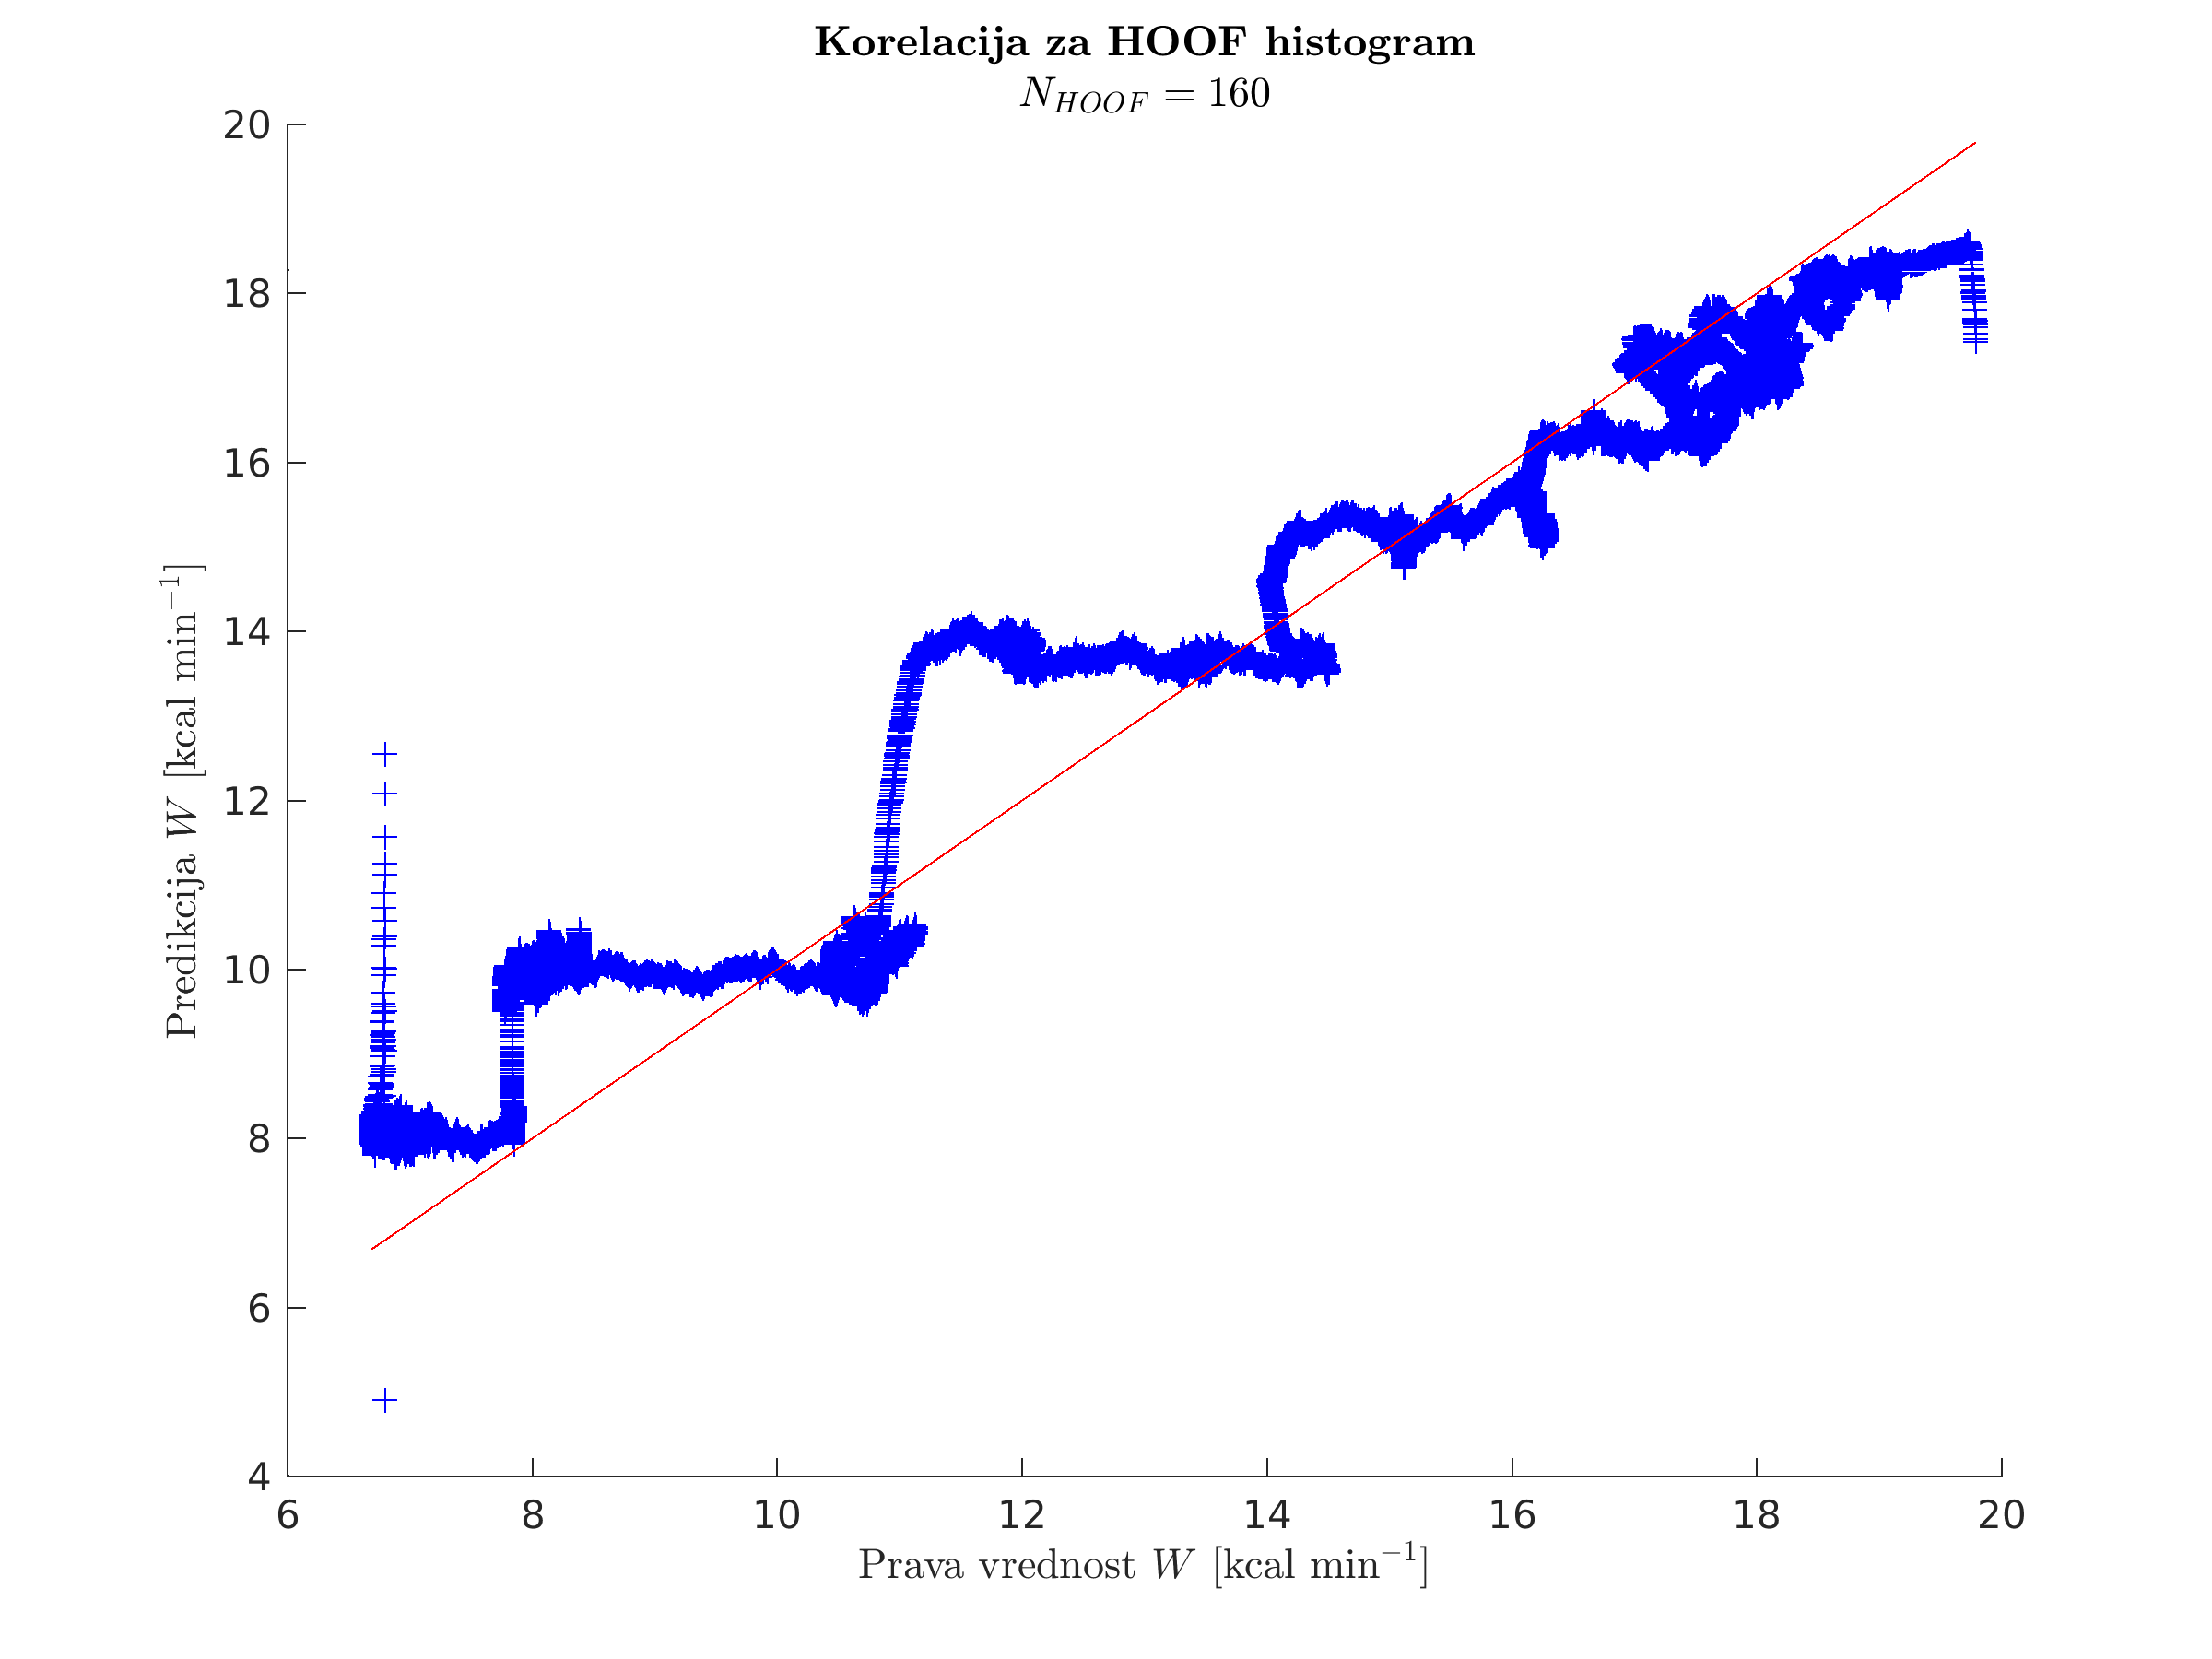
\includegraphics[width=\columnwidth]{./Slike/corr-hafa-160.png}
      \caption{Korelacija $N_{HAFA}=160$.}
      \label{fig:corr-hafa-160}
    \end{subfigure}
    \caption[Grafi korelacij modelov z različnim $N_{HAFA}$]{Grafi korelacij modelov z različnim številom stolpcev $N_{HAFA}$ HAFA deskriptorja. Rezultati so si zelo podobni.}
    \label{fig:corr-hafa}
\end{figure}










\subsection{Izbira deskriptorjev}

Chaudhry et al. \cite{chaudhry2009histograms} predlaga uporabo histogramov orientiranega optičnega toka (HOOF) za estimacijo gibanja. Vendar pa smo v preliminarnih terenskih testiranjih \cite{koporec2017observation} ugotovili, da njihova uporaba v realnih okoliščinah ni zadovoljiva. HOOF deskriptorju smo pripeli HAFA deskriptor in tako dobili razširjeni deskriptor HOOF-HAFA, ki v splošnem daje boljše rezultate, kot lahko vidimo v tabeli \ref{tab:izbira} in na primerjalnih slikah \ref{fig:izbira}.

Pri evaluaciji deskriptorjev HOOF in HOOF-HAFA smo uporabili učne vzorce hrbtne kamere terenskih testov. Evaluirali smo za podatke srčnega utripa $hr$. Srčni utrip smo za gradnjo modelov pretvorili v energijsko porabo $W$ po enačbi \eqref{eq:charlot}. Pridobljene značilke smo normirali na intervalu [0,1] in jih uporabili za učenje regresijskega modela z metodo podpornih vektorjev $\epsilon$-SVR in jedrom RBF. Za določitev optimalnih parametrov, ki so predstavljeni v tabeli \ref{tab:nhoof-param}, smo uporabili optimizacijsko metodo mrežnega iskanja \cite{hsu2003practical}. Rezultate smo filtrirali še s Gaussovim jedrom (predstavljen v \ref{sec:gaussov-filter}) velikosti $6$ in varianco $\sigma=16$. 

\begin{table}[htb]
	\centering
    \begin{tabular}{l S[table-format=2.3] S[table-format=1.3] S[table-format=1.3] S[table-format=1.3]}
    \toprule
    \thead{Deskriptor} & \thead{$\mathbf{C}$} & \thead{$\mathbf{\gamma}$} & \thead{$\mathbf{\epsilon}$} & \thead{MSE} \\ 
    \midrule
    HOOF & 2.828 & 11.314 & 0.435 & 2.192 \\
    HOOF-HAFA & 5.657 & 2.828 & 0.154 & 1.781 \\
    \bottomrule
    \end{tabular}
    \caption[Optimalni parameteri RBF jedra modelov za izbiro deskriptorjev]{Optimalni parametri RBF jedra za modele z različnim deskriptorjem.}
    \label{tab:izbira-param}
\end{table}


\begin{table}[htb]
	\centering
    \begin{tabular}{l S[table-format=1.3] S[table-format=1.3] S[table-format=1.3] S[table-format=2.2]}
    \toprule
    \thead{Deskriptor} & \thead{$r$} & \thead{RAE} & \thead{RMSE} & \thead{nSV [\%]}\\
    \midrule%nSV
    HOOF & 0.992 & 0.336 & 0.317 & \boldentry{2.2}{82.34} \\%2187/2656
    \textbf{HOOF-HAFA} & \boldentry{1.3}{0.991} & \boldentry{1.3}{0.157} & \boldentry{1.3}{0.205} & 89.53 \\%2378
    \bottomrule
    \end{tabular}
    \caption[Rezultati evaluacije modelov z različnim deskriptorjem]{Rezultati evaluacije modelov z različnim deskriptorjem. Optimalni rezultati so odebeljeni. Vidimo lahko, da se bolje odnese razširjeni deskriptor HOOF-HAFA, čeprav model uporablja več podpornih vektorjev. }
    \label{tab:izbira}
\end{table}



\begin{figure}[htb]
	\centering
    \begin{subfigure}[t]{0.45\columnwidth}
      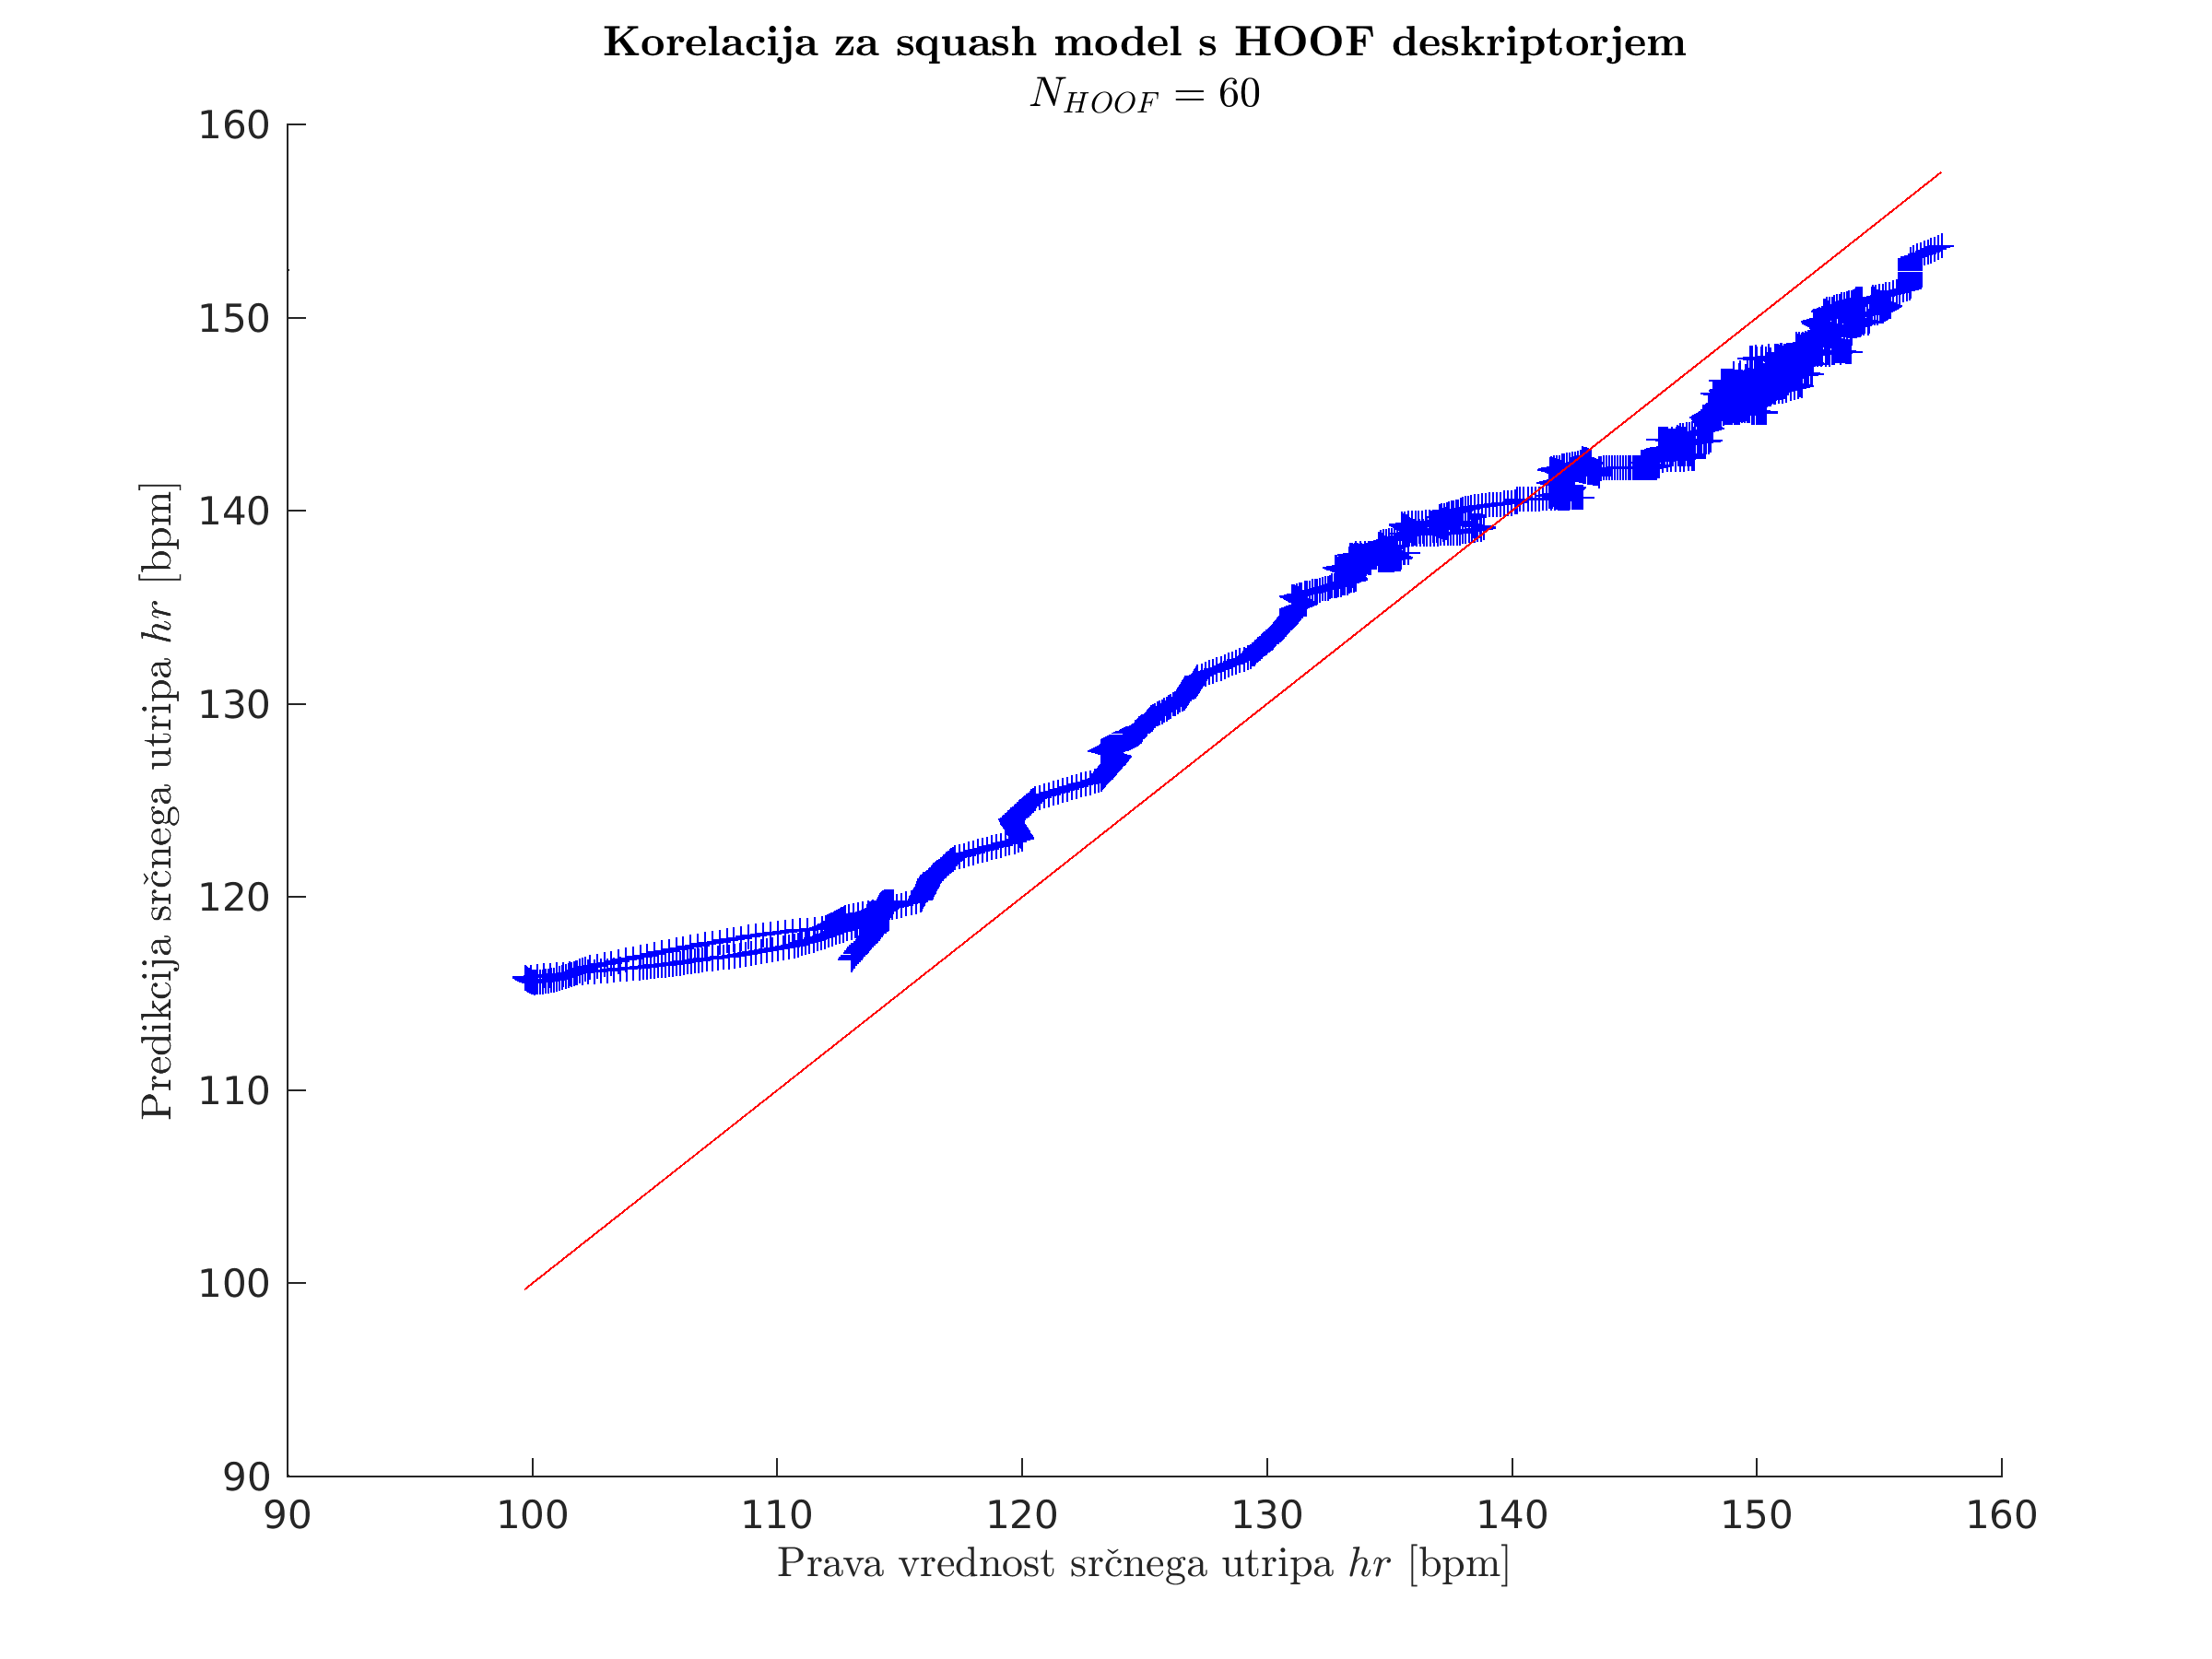
\includegraphics[width=\columnwidth]{./Slike/corr-hoof.png}
      \caption{Korelacija $N_{HOOF}=60$.}
      \label{fig:izbira-hoof}
    \end{subfigure}
    ~
    \begin{subfigure}[t]{0.45\columnwidth}
      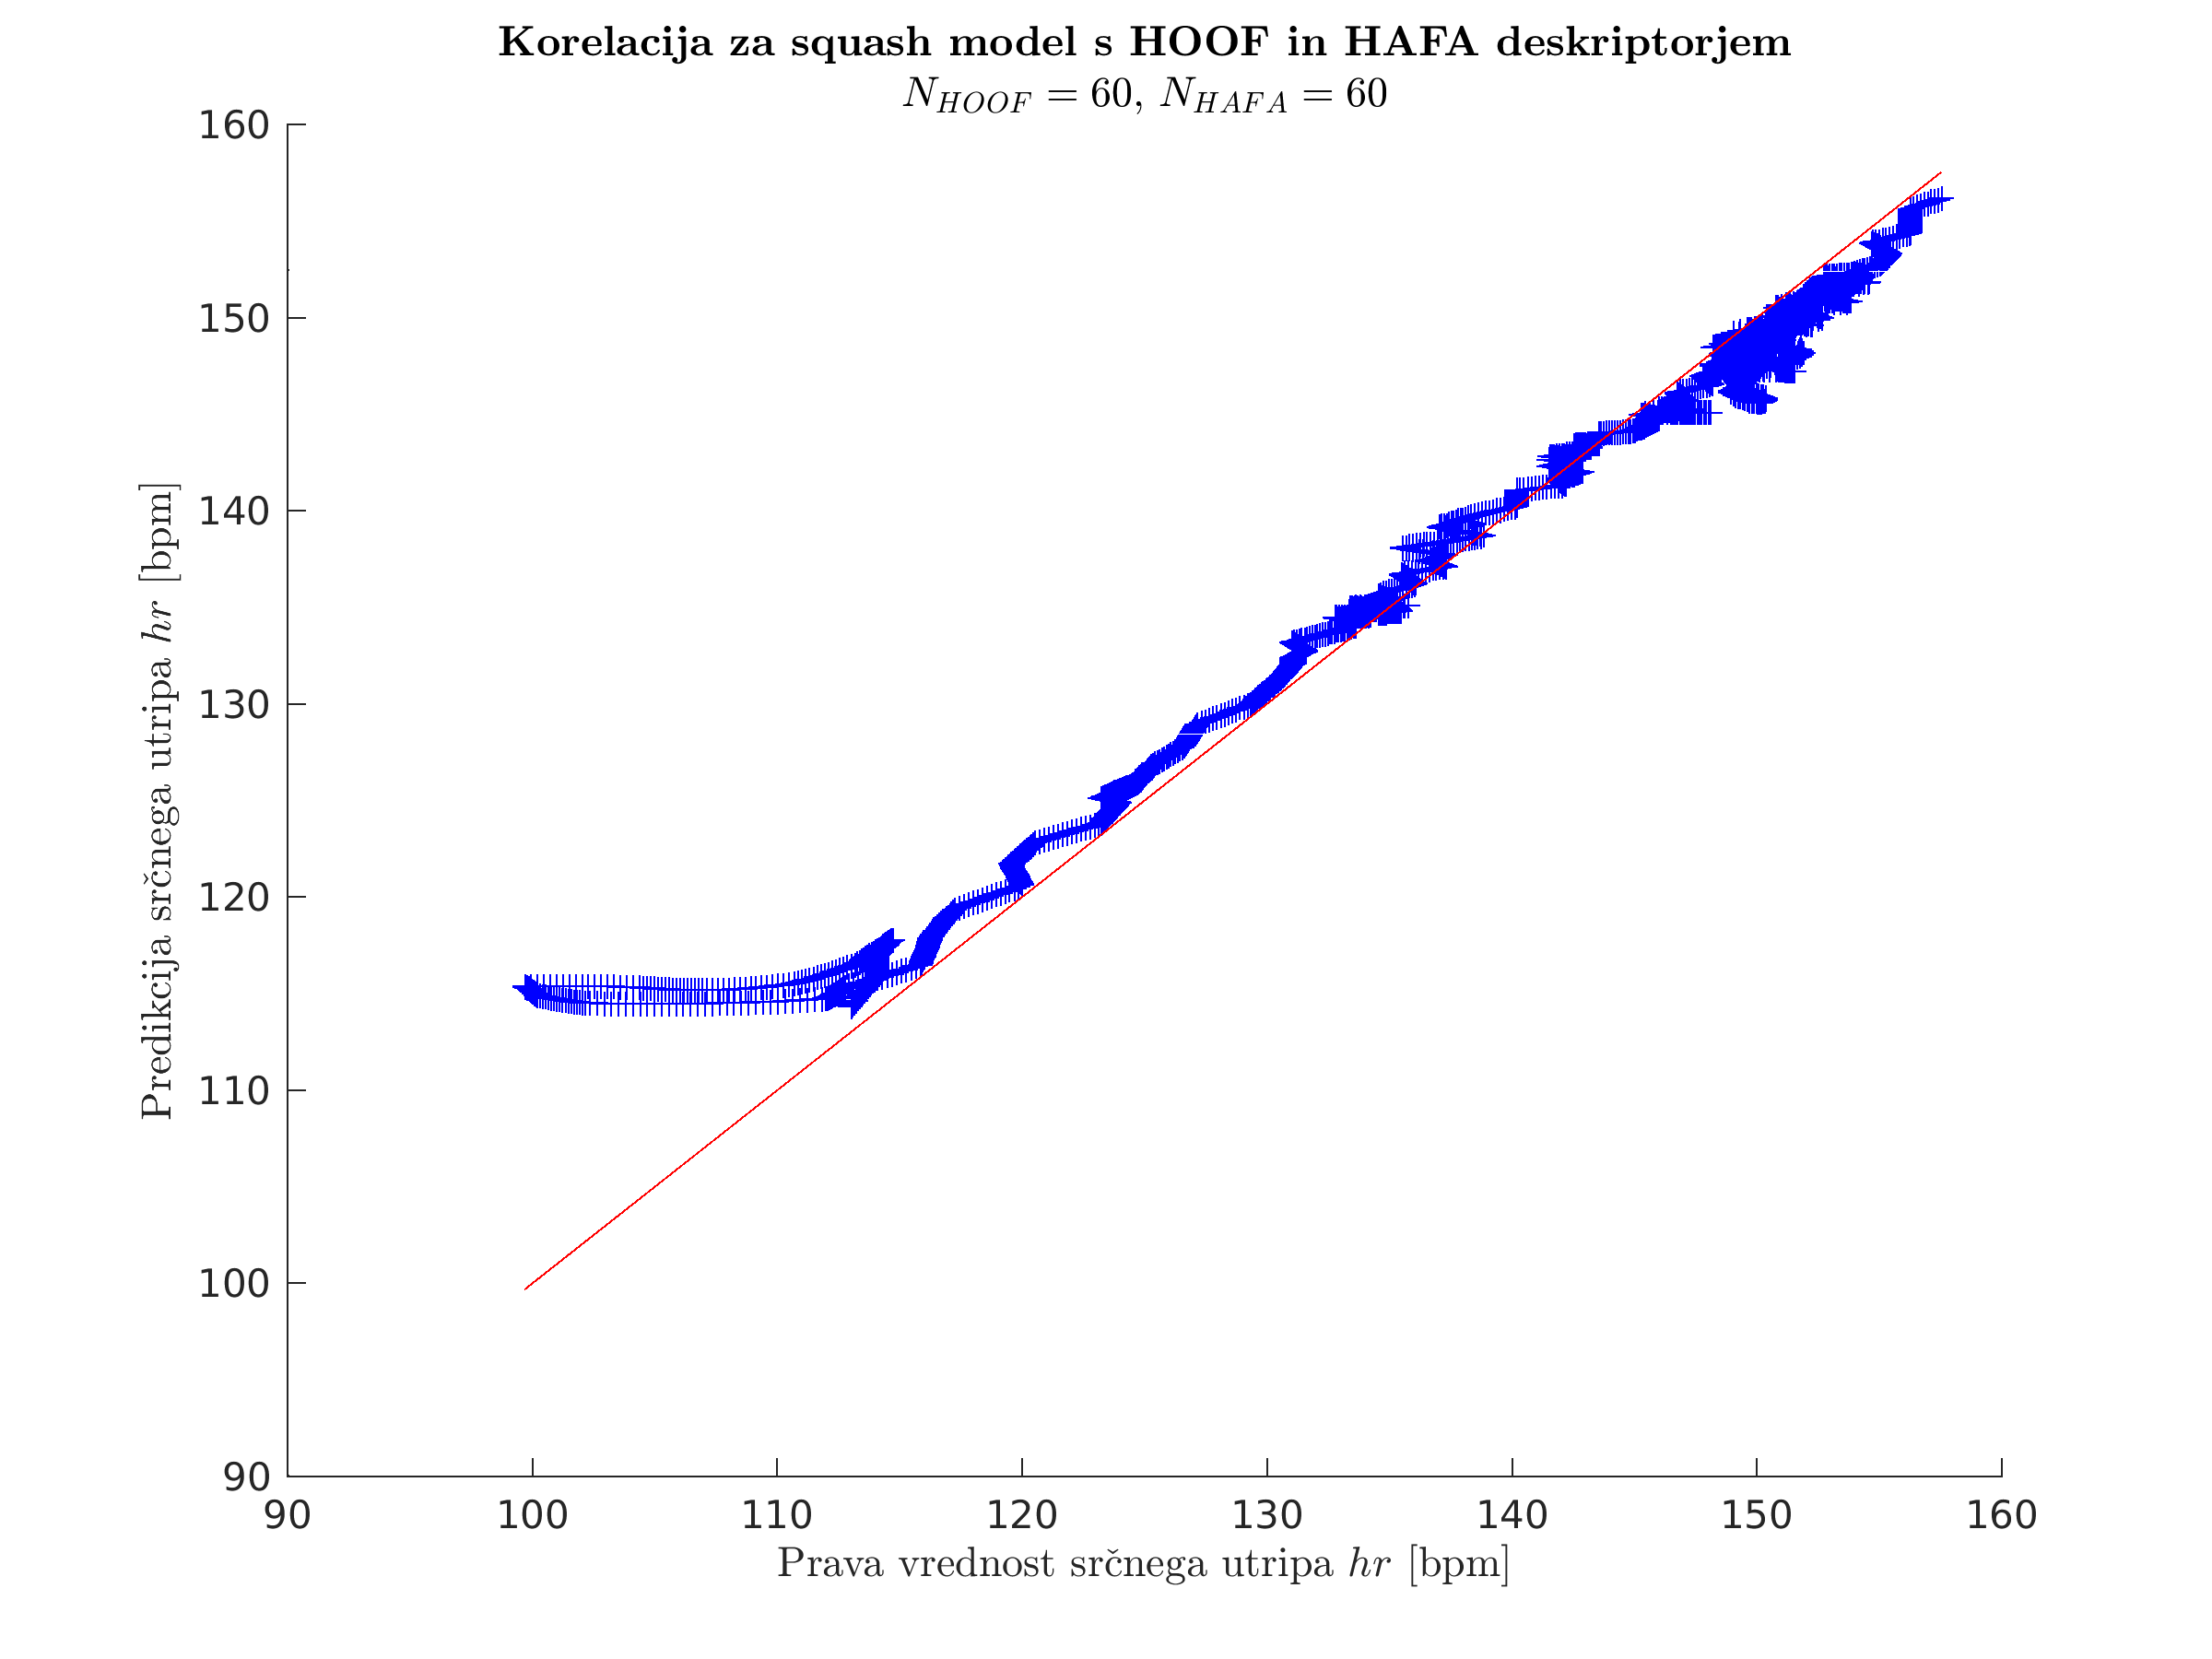
\includegraphics[width=\columnwidth]{./Slike/corr-hoof-hafa.png}
      \caption{Korelacija $N_{HOOF}=60$,\\$N_{HAFA}=60$.}
      \label{fig:izbira-hoofhafa}
    \end{subfigure}
    \caption[Primerjava modelov s HOOF in HOOF-HAFA deskriptorji]{Primerjava grafov korelacij modelov z različnimi deskriptorji. Model \subref{fig:izbira-hoof}) smo naučili s HOOF deskriptorjem. Model \subref{fig:izbira-hoofhafa}) smo naučili s HOOF in HAFA deskriptorjem. Posamezen vzorec je tako vseboval $120$ značilk. Pri primerjavi korelacije lahko opazimo vidno razliko. Model \subref{fig:izbira-hoofhafa}) dokazuje, da je razširjeni deskriptor boljši.}
    \label{fig:izbira}
\end{figure}




